% Options for packages loaded elsewhere
\PassOptionsToPackage{unicode}{hyperref}
\PassOptionsToPackage{hyphens}{url}
%
\documentclass[
]{article}
\usepackage{amsmath,amssymb}
\usepackage{iftex}
\ifPDFTeX
  \usepackage[T1]{fontenc}
  \usepackage[utf8]{inputenc}
  \usepackage{textcomp} % provide euro and other symbols
\else % if luatex or xetex
  \usepackage{unicode-math} % this also loads fontspec
  \defaultfontfeatures{Scale=MatchLowercase}
  \defaultfontfeatures[\rmfamily]{Ligatures=TeX,Scale=1}
\fi
\usepackage{lmodern}
\ifPDFTeX\else
  % xetex/luatex font selection
\fi
% Use upquote if available, for straight quotes in verbatim environments
\IfFileExists{upquote.sty}{\usepackage{upquote}}{}
\IfFileExists{microtype.sty}{% use microtype if available
  \usepackage[]{microtype}
  \UseMicrotypeSet[protrusion]{basicmath} % disable protrusion for tt fonts
}{}
\makeatletter
\@ifundefined{KOMAClassName}{% if non-KOMA class
  \IfFileExists{parskip.sty}{%
    \usepackage{parskip}
  }{% else
    \setlength{\parindent}{0pt}
    \setlength{\parskip}{6pt plus 2pt minus 1pt}}
}{% if KOMA class
  \KOMAoptions{parskip=half}}
\makeatother
\usepackage{xcolor}
\usepackage[margin=1in]{geometry}
\usepackage{graphicx}
\makeatletter
\def\maxwidth{\ifdim\Gin@nat@width>\linewidth\linewidth\else\Gin@nat@width\fi}
\def\maxheight{\ifdim\Gin@nat@height>\textheight\textheight\else\Gin@nat@height\fi}
\makeatother
% Scale images if necessary, so that they will not overflow the page
% margins by default, and it is still possible to overwrite the defaults
% using explicit options in \includegraphics[width, height, ...]{}
\setkeys{Gin}{width=\maxwidth,height=\maxheight,keepaspectratio}
% Set default figure placement to htbp
\makeatletter
\def\fps@figure{htbp}
\makeatother
\setlength{\emergencystretch}{3em} % prevent overfull lines
\providecommand{\tightlist}{%
  \setlength{\itemsep}{0pt}\setlength{\parskip}{0pt}}
\setcounter{secnumdepth}{-\maxdimen} % remove section numbering
% definitions for citeproc citations
\NewDocumentCommand\citeproctext{}{}
\NewDocumentCommand\citeproc{mm}{%
  \begingroup\def\citeproctext{#2}\cite{#1}\endgroup}
\makeatletter
 % allow citations to break across lines
 \let\@cite@ofmt\@firstofone
 % avoid brackets around text for \cite:
 \def\@biblabel#1{}
 \def\@cite#1#2{{#1\if@tempswa , #2\fi}}
\makeatother
\newlength{\cslhangindent}
\setlength{\cslhangindent}{1.5em}
\newlength{\csllabelwidth}
\setlength{\csllabelwidth}{3em}
\newenvironment{CSLReferences}[2] % #1 hanging-indent, #2 entry-spacing
 {\begin{list}{}{%
  \setlength{\itemindent}{0pt}
  \setlength{\leftmargin}{0pt}
  \setlength{\parsep}{0pt}
  % turn on hanging indent if param 1 is 1
  \ifodd #1
   \setlength{\leftmargin}{\cslhangindent}
   \setlength{\itemindent}{-1\cslhangindent}
  \fi
  % set entry spacing
  \setlength{\itemsep}{#2\baselineskip}}}
 {\end{list}}
\usepackage{calc}
\newcommand{\CSLBlock}[1]{\hfill\break\parbox[t]{\linewidth}{\strut\ignorespaces#1\strut}}
\newcommand{\CSLLeftMargin}[1]{\parbox[t]{\csllabelwidth}{\strut#1\strut}}
\newcommand{\CSLRightInline}[1]{\parbox[t]{\linewidth - \csllabelwidth}{\strut#1\strut}}
\newcommand{\CSLIndent}[1]{\hspace{\cslhangindent}#1}
\ifLuaTeX
  \usepackage{selnolig}  % disable illegal ligatures
\fi
\usepackage{bookmark}
\IfFileExists{xurl.sty}{\usepackage{xurl}}{} % add URL line breaks if available
\urlstyle{same}
\hypersetup{
  pdftitle={Agroecological Importance of Smooth Brome in Managing Wheat Stem Sawfly (Hymenoptera: Cephidae) via Its Associated Braconid Parasitoids},
  hidelinks,
  pdfcreator={LaTeX via pandoc}}

\title{Agroecological Importance of Smooth Brome in Managing Wheat Stem
Sawfly (Hymenoptera: Cephidae) via Its Associated Braconid Parasitoids}
\author{}
\date{\vspace{-2.5em}2024-06-06}

\begin{document}
\maketitle

This document can be downloaded as either a .docx or .pdf document.
Please be aware that conversion may cause the formatting to be altered.

Download .docx

Download .pdf

\subsection{Abstract}\label{abstract}

Wheat stem sawfly, \emph{Cephus cinctus} Norton (WSS), causes
significant damage in cereal crops throughout the Northern Great Plains
of North America. Bracon cephi and Bracon lissogaster are native WSS
parasitoids important in managing WSS outbreaks and damage. Smooth Brome
(Bromus inermis) grass has been found to be an effective parasitoid
sink, and potential trap crop, when grown in areas surrounding wheat
fields in Montana. As climate changes continue to alter central and
northern Montana, WSS will continue to cause immense damage to dry-land
cereal crop yields. My study observes the utilization of smooth brome in
providing year-over-year host refuge for Bracon spp. We measured the WSS
larval survival rate within controlled smooth brome plots, observing a
maximum end-of-year survival of 5.7\%. We also collected stems from
central and northern Montana where we measured the WSS infestation and
parasitoid prevalence within cultivated wheat and adjacent smooth brome.
Montana fields sites showed similar high year-end WSS larval mortality
while showcasing high levels of parasitism. This research underlines the
importance of providing a sustainable ecological buffer for WSS
parasitoids as climate conditions continue to change.

\subsection{Introduction}\label{introduction}

Ecologists and farmers frequently hold divergent views regarding the
importance of natural habitats within agricultural landscapes, a
distinction often overlooked in ecological and conservation discourse
(\citeproc{ref-Tscharntke2016}{Tscharntke et al. 2016}). While
ecologists recognize the role of natural habitats such as field border
vegetation in supporting biodiversity and providing potential ecosystem
services like biological pest control, many farmers perceive these
semi-arid habitat remnants as occupying valuable cropland or even as
sources of pests. As such, documenting how pest and natural enemy
populations interact with agricultural landscapes alongside semi-natural
habitat buffers on the crop periphery is important in determining the
degree of the services or disservices provided.

Numerous polyphagous insect herbivores and their natural enemies rely on
a variety of resources found across diverse habitat types within their
environment. Depending upon the quality of the resource, different
habitat types can serve as sources for increased pest or natural enemy
populations. Similarly, these habitat types can serve as sinks that
decrease populations (\citeproc{ref-Kennedy2000}{Kennedy and Storer
2000}). Altering the presence of these resources can have impacts on
pest or natural enemy populations and can alter the ecology between the
examined species. For example, diversifying the edge cropping of organic
\emph{Brassica} using fava beans, fennel, and marigolds results in a
diversity in beneficial arthropod communities that help reduce
phytophagous herbivory (\citeproc{ref-DeMorais2023}{Morais et al.
2023}).

Understanding the ways in which landscape habitat diversity impacts the
ecological relationship between pest and enemy is crucial for
effectively managing pest species in large scale cropping systems.
Similarly, understanding how herbivore plant-hosts act as reservoirs for
pests or beneficial natural enemies can potentially play a role in
stabilizing year-over-year agricultural impact from these pests
(\citeproc{ref-Cano2022}{Cano et al. 2022}).

The wheat stem sawfly (WSS), Hymenoptera \emph{Cephus cinctus} Norton,
is a grass-mining sawfly native to North America {[}Criddle
(\citeproc{ref-Criddle1922}{1922}); Ainslie1929; Wallace and McNeal
(\citeproc{ref-Wallace1966}{1966}); Lesieur et al.
(\citeproc{ref-Lesieur2016}{2016}){]}. Originally adept at utilizing
wild grass hosts, the species became a major pest to cultivated cereals
as this resource became more prevalent following European settlement,
becoming a notable pest of winter wheat in 1990 in Montana
(\citeproc{ref-Morrill1996}{Morrill and Kushnak 1996}), and more
recently in Colorado (\citeproc{ref-Cockrell2021}{Cockrell et al.
2021}). Climate warming has the potential to further expand the range of
this pest both northward and southward (\citeproc{ref-Olfert2019}{Olfert
et al. 2019}, \citeproc{ref-Weaver2023}{Weaver 2023}). Adult female WSS
use their saw-like ovipositor to lay their eggs in the lumen of stems,
where the eggs hatch, leading to larval feeding of parenchyma tissue
{[}Roemhild1954; Holmes and Farstad
(\citeproc{ref-Holmes1956}{1956}){]}. Economic damage manifests in the
form of both kernel weight reduction caused by tissue damage {[}Beres et
al. (\citeproc{ref-Beres2011a}{2011}); Delaney2010{]} and stem toppling
due to late-season larval girdling (\citeproc{ref-Holmes1960}{Holmes and
Peterson 1960}, \citeproc{ref-Nansen2005a}{Nansen et al. 2005},
\citeproc{ref-McCullough2020}{McCullough et al. 2020}).

Several parasitoid or predatory species attack \emph{C. cinctus} within
wild grass hosts Morrill et al. (\citeproc{ref-Morrill2001}{2001}),
however, two species, \emph{Bracon cephis} (Gahan) and \emph{Bracon
lissogaster} Muesebeck (Hymenoptera: Braconidae), have been observed
targeting WSS within cultivated cereals
(\citeproc{ref-Nelson1953}{Nelson and Farstad 1953},
\citeproc{ref-Morrill1998}{Morrill et al. 1998},
\citeproc{ref-Runyon2001a}{Runyon et al. 2001},
\citeproc{ref-Runyon2001b}{Runyon 2001}). These two host-specific
ectoparasitoids are native to North America. Both parasitoids are
bivoltine, with the first generation present in Montana from late-June
to late-July, while the second generation is active from mid-July to
September (\citeproc{ref-Gahan1918}{Gahan 1918},
\citeproc{ref-Somsen1956}{Somsen and Luginbill 1956},
\citeproc{ref-Davis2013}{Davis 2013}). Adult female \emph{B. cephi} and
\emph{B. lissogaster} inject a paralytic toxin into a \emph{C. cinctus}
larvae within the host stem, paralyzing the host larvae, and depositing
from a single (\emph{B. cephi}) to 1-3 (\emph{B. lissogaster}) eggs.
\emph{B. cephi} and \emph{B. lissogaster} have been shown to provide
biological control via irreplaceable mortality of \emph{C. cinctus}
populations (\citeproc{ref-Peterson2011}{Peterson et al. 2011},
\citeproc{ref-Buteler2015}{Buteler et al. 2015}) and can significantly
reduce \emph{C. cinctus} damage and impact on crop yields
(\citeproc{ref-Buteler2008}{Buteler et al. 2008},
\citeproc{ref-Bekkerman2018}{Bekkerman and Weaver 2018},
\citeproc{ref-Adhikari2019}{Adhikari et al. 2019},
\citeproc{ref-Rand2020}{Rand et al. 2020}). While \emph{C. cinctus} has
a wide range of viable host plants, including native and non-native
grasses and cultivated row-crops such as wheat (\emph{Triticum aestivum
L.}) and barley (\emph{Hordeum vulgare})
(\citeproc{ref-Wallace1966}{Wallace and McNeal 1966},
\citeproc{ref-Cockrell2017}{Cockrell et al. 2017},
\citeproc{ref-Achhami2020}{Achhami et al. 2020}), infestation levels can
vary widely across hosts. Previous research has shown preference for
host plants with larger stem diameter
(\citeproc{ref-Ainslie1920}{Ainslie 1920},
\citeproc{ref-Buteler2009}{Buteler et al. 2009},
\citeproc{ref-Bhandari2020}{Bhandari 2020}).

Recent research has shown natural non-cultivated grasses such as
\emph{Agropyron cristatum}, \emph{Bromus techtorum}, \emph{Bromus
inermis}, \emph{Elymus trachycaulus}, and \emph{Thinopyrum intermedium}
host \emph{C. cinctus} and most also host Bracon spp. parasitoids quite
well (\citeproc{ref-Mendoza2006}{Perez-Mendoza and Weaver 2006},
\citeproc{ref-Peirce2021}{Peirce et al. 2021},
\citeproc{ref-Rand2024}{Rand et al. 2024}). We find investigating
\emph{B. inermis} holds the most potential, as it has been shown to be a
quality initially-accepted host for \emph{C. cinctus} oviposition while
also leading to high larval mortality later on
(\citeproc{ref-Seamans1928}{Seamans 1928},
\citeproc{ref-Farstad1945}{Farstad and Jacobson 1945}). However, there
is a lack of detailed relating to the total infestation, cutting, and
parasitism within \emph{B. inermis} at multiple time points throughout
the growing season. Quantitative assessment of potential `reservoir'
characteristics and local spatial information could prove useful in
fully understanding the ecological impacts of maintaining \emph{B.
inermis} along roadways and within coulees.

Smooth brome (\emph{Bromus inermis} Leyss) is a Eurasian cool-season
rhizomatous grass introduced to the United States in 1884
(\citeproc{ref-Bolwahn2011}{Salesman and Thomsen 2011}).\emph{B.
inermis} was originally thought of as potentially useful as a trap crop
in order to combat the growing WSS problem with cultural control
practices (\citeproc{ref-Criddle1922}{Criddle 1922},
\citeproc{ref-Farstad1945}{Farstad and Jacobson 1945},
\citeproc{ref-Beres2011a}{Beres et al. 2011}). Due to its low
agricultural value, and propensity to form monocultures and out compete
many native grasses, \emph{B. inermis} is categorized as invasive in
some habitats (\citeproc{ref-Carlson1985}{Carlson and Newell 1985},
\citeproc{ref-Willson2000}{Willson and Stubbendieck 2000},
\citeproc{ref-Dillemuth2008}{Dillemuth et al. 2008}). However, \emph{B.
inermis} still holds considerable ecological and potential economic
value due to its late senescence and WSS antibiosis properties
(\citeproc{ref-Otfinowski2006}{Otfinowski et al. 2006},
\citeproc{ref-Rand2024}{Rand et al. 2024}).

Montana's golden triangle, an area of central and northern Montana with
intense cereal grain production, is prone to drought and burning via
wildfire (\citeproc{ref-Wilson1923}{Wilson 1923},
\citeproc{ref-Adhikari2019}{Adhikari et al. 2019}). As both \emph{C.
cinctus} and its host-specific parasitoids are relatively restricted in
their annual mobility (\citeproc{ref-Weaver2005}{\textbf{Weaver2005?}}),
environmental extremes can have broad impacts on both local pest and
natural enemy populations. As with many predator-prey interactions, the
\emph{C. cinctus} and parasitoid populations fluctuate, with crashes and
spikes experienced in close succession and through ineteraction with
drought (\citeproc{ref-Holmes1963}{Holmes et al. 1963},
\citeproc{ref-Holmes1982}{Holmes 1982}). Similar examples of these
classical population dynamics patterns can be found in wolves and moose
on Isle Royale (\citeproc{ref-Peterson1999}{Peterson 1999}), and
Coccinellidae and aphids (\citeproc{ref-Evans1999}{Evans 1999}), among
others.

We examined historical weather data from two field locations (10 sites
overall) in central and northern Montana. We used this data to
understand how changes in global climate trends may be impacting
\emph{C. cinctus}, \emph{B. cephi} and \emph{B. lissogaster} interact
with \emph{B. inermis} populations. In addition we analyzed normalized
difference vegetative index (NDVI) at our field sites to understand how
\emph{B. inermis} senescence patterns compare to adjacent cultivated
wheat fields.

In this study, we explored the ecological patterns between Montana
populations of \emph{C. cinctus} and its associated braconid parasitoids
in relation to \emph{B. inermis} host sites. Our goal, was 1) to
understand the degree to which \emph{C. cinctus} infested \emph{B.
inermis} stems in relation to neighboring cereal crops, and 2) the way
in which braconid parasitoids utilized WSS hosts available within
\emph{B. inermis} stems. To do so, we conducted two separate studies. In
our first study, we conducted controlled \emph{C. cinctus} infestation
of \emph{B. inermis} to understand the relative infestation and cutting
rate of \emph{C. cinctus} within the \emph{B. inermis} stems in the
absence of parasitoids. The second study examined rates of cutting and
parasitism in wheat crops and their surroundings at field sites in
central and northern Montana.

Using these studies, we addressed three questions, 1) what is the total
\emph{C. cinctus}-caused stem cutting heading into overwinter - and thus
the source rate, of the subsequent \emph{C. cinctus} population in
\emph{B. inermis}? 2) can \emph{C. cinctus} larvae within \emph{B.
inermis} serve as critical second generation hosts for \emph{B. cephi}
and \emph{B. lissogaster}? and 3) how do annual \emph{C. cinctus} and
parasitoid populations in \emph{B. inermis} compare with those in the
adjacent cultivated wheat fields?

\subsection{Materials and Methods}\label{materials-and-methods}

All data for experiments was analyzed using R Studio (R Studio version
2024.04.0+735, R 2024).

\subsubsection{Weather data and NDVI
analysis}\label{weather-data-and-ndvi-analysis}

\emph{Weather data.} We assessed the medium- and long-term temperature
and precipitation trends of our field sites using weather data from the
National Oceanic and Atmospheric Administration (NOAA, Silver Spring,
MA, USA). Data for each field site was averaged from three of the
closest weather stations to that location. Data was plotted using R
package `ggplot' (version 3.4.4) (\citeproc{ref-ggplot}{Wickham 2016}).
Data was then fit using a linear model using the `lm' command using
average yearly precipitation (inches) as the response variable and year
as the predictor.

\emph{NDVI analysis.} We compared the relative greening throughout the
growing season between wheat fields and adjacent \emph{B. inermis} using
the normalized difference vegetation index (NDVI). NDVI is typically
used to assess vegetation health and density, and is calculated from the
visible and near-infrared light reflected by vegetation
(\citeproc{ref-Pettorelli2005}{Pettorelli et al. 2005}). NDVI data
measurements were directly downloaded using Google Earth Engine (Google
Inc.~2023, Mountain View, CA, USA). Similar to our weather data
analysis, NDVI data was modeled using the linear modeling package `lm'
in R to discern differences in NDVI measurments over time.

\subsubsection{\texorpdfstring{Controlled \emph{C. cinctus} infestation
of \emph{B.
inermis}}{Controlled C. cinctus infestation of B. inermis}}\label{controlled-c.-cinctus-infestation-of-b.-inermis}

\emph{Insects and Cages.} Assessment of \emph{C. cinctus} infestation
and mortality within \emph{B. inermis} were assessed using a 34 x 60 ft
plot at the Arthur H. Post Agronomy Farm (43°38'19.39''N,
116°14'28.86''W), an experimental farm of Montana State University in
Bozeman, MT. There is a negligible population of \emph{C. cinctus} and
associated parasitoids at this location. Experimental cages were built
using 1-inch PVC piping with the netting made using 530\(\mu\) Amber
Lumite Screen (BioQuip\(^\circledR\) Products, LLC). Twelve cages were
built to dimensions of 6ft x 3ft x 3ft (L x W x H) with cage locations
selected randomly based on the space available within the plot and
arranged in sets of three.

Wheat stem stubble was collected in Three Forks, MT, USA
(43°38'19.39''N, 116°14'28.86''W) from fields that experienced high
levels of \emph{C. cinctus} infestation and cutting the year prior, as
previously described (\citeproc{ref-Hager2024}{Hager et al. 2024}). Cut
stubble, which contained \emph{C. cinctus} larvae in diapause, were kept
refrigerated between -2°C and 3°C for \textgreater100 days as required
to complete obligatory larval diapause. As needed, stubs were removed
from refrigeration and kept at 22-27°C for 4-5 weeks inside of 100 oz
GladWare® storage containers (Glad®, Oakland, California USA). Once
\emph{B. inermis} stems reached six inches tall, stub containers with
emerging sawflies were added to cages to mimic sawfly infestation
pressure. Sawfly quantity treatments were as follows: high (600 stubs),
low (200 stubs), and control (0 stubs).

\emph{Data Collection.} In late August, \emph{B. inermis} stems were
collected from each cage. Each stem was sliced open using X-Acto® knives
to collect data on infestation, dead larvae and live larvae, as well as
very rare parasitism events, for each internode.

\subsubsection{Montana Field Survey}\label{montana-field-survey}

\emph{Stem collection and processing.} We conducted a field survey to
assess \emph{C. cinctus} infestation, larval mortality, and \emph{B.
cephi} and \emph{B. lissogaster} prevalence within \emph{B. inermis} and
adjacent wheat fields. Sites were chosen across 2 counties in
north-central Montana, United States. (Chouteau, Judith Basin), which
consistently experience high \emph{C. cinctus} pressure. Samples were
collected from wheat fields and adjacent \emph{B. inermis} in early July
and late August in 2022, and 2023 from sites in Big Sandy and Moccasin
MT, USA. Sampling sites were set up as 100\(m^2\) polygons along the
edge of adjoining wheat fields. Four collection squares of 1ft x 1ft
were randomly selected within each polygon during both collection events
each year. All stems within each 1 x 1 ft square were collected using a
shovel to remove both stem and root material. Wheat stems were collected
at distances of 5 and 20 meters from the edge of the field. Samples were
collected in 4 rows at 10 meters apart. 2 samples were collected in each
row at distances of 5 and 20 meters. 1 ft samples were collected at each
point.

Wheat and \emph{B. inermis} stems were then returned to Montana State
University, Bozeman, Montana and stored in a 10°C cold, humid storage
until dissection. Stems were dissected in the same manner as samples
from our controlled experiment. We recorded presence or absence of
\emph{C. cinctus} larval infestation, live eggs, dead eggs, dead larvae,
live larvae and parasitism, in addition to stem cutting. Sawfly larvae
were identified based on descriptions in Criddle (1915) and Wallace and
McNeal (1996).

\emph{Statistical Analysis.} We used generalized linear mixed models
with binomial errors (logit link) fit using bound optimization by
quadratic approximation, with a maximum of 200,000 iterations, were run
in the \emph{lme4} package in R (\citeproc{ref-lme4}{Bates et al. 2015})
to examine the effects of location and year (fixed effects) on each of
the three response variables: proportion of stems infested, proportion
of stems cut, and proportion of stems parasitized by \emph{Bracon} spp.

To better understand the densities of host \emph{C. cinctus} and the
\emph{Bracon} spp. within the wheat and adjacent \emph{B. inermis} at
each sampling site, we converted our units to the ratio of parasitoids
to surviving hosts stem per unit area. Densities of stems are different
when considering semi-natural, long-standing stands of \emph{B. inermis}
and the adjacent cultivated wheat or barley.

\subsection{Results}\label{results}

\subsubsection{Historical Weather Analysis \&
NDVI}\label{historical-weather-analysis-ndvi}

We observed a significant linear relationship (\emph{r = 0.1, P = 0.033,
estimate = -0.058}) between average precipitation and year for both Big
Sandy and Moccasin, Montana. For each location and one-year increase, we
observed a 0.05 inch decrease in precipitation. (\hyperref[figure1]{Fig.
1}). Additionally, we observed a significant positive linear
relationship (\emph{r = 0.245, P \textless{} 0.05, estimate = 0.028})
between year and average yearly temperature for Moccasin and Big Sandy,
MT. Thus, each year, the average daily temperature has increased by
0.03°C. (\hyperref[figure2]{Fig. 2}).

We observed a notable difference in NDVI when comparing adjacent
\emph{B. inermis} and spring wheat. We saw a significant difference in
the July NDVI (\emph{0.846, P \textless{} 0.05}). The \emph{B. inermis}
NDVI remained relatively linear in it's downslope (BROME SLOPE POST
JULY) compared to the wheat field (WHEAT FIELD POST JULY).
(\hyperref[figure3]{Fig. 3})

Need to add map showing where NDVI measurements came from

\subsubsection{\texorpdfstring{Controlled \emph{C. cinctus} Infestation
of \emph{B.
inermis}}{Controlled C. cinctus Infestation of B. inermis}}\label{controlled-c.-cinctus-infestation-of-b.-inermis-1}

Initially, \emph{C. cinctus} heavily infested stems of \emph{B. inermis}
in the controlled test conditions. Averaged across both years, we
observed 66.5\% of stems infested for high treatments and 47.3\% of
stems for low treatments. We found strong evidence suggesting that there
was a significant difference between infestation at high and low
treatment levels when holding year constant (\emph{r = 0.83, P
\textless{} 0.05}, \hyperref[figure4]{Fig. 3}).

Stem cutting by mature larvae, leading into winter, was observed at
5.7\% for the high treatments and 3.9\% for the low, showing strong
evidence for a difference in cutting between high and low treatment
groups (\emph{r = 0.592, P \textless{} 0.05}). There was a dramatic
decrease in survival observed from initial infestation to stem cutting.

\emph{C. cinctus} infested stems often contained larvae burrowing
through multiple nodes. In 2022, 64.3\% of stems were observed to have
at least 4 nodes burrowed through, or 5 internodes occupied. In 2023,
61.7\% of stems had at least 4 nodes infested \hyperref[figure5]{Fig. 5}

\subsubsection{Montana Field Sites}\label{montana-field-sites}

We quantified \emph{C. cinctus} and \emph{Bracon} spp. parasitoid
presence in 6,148 wheat and grass stems across 10 research sites in 2022
and 2023. Initial infestation of \emph{B. inermis} by \emph{C. cinctus}
varied between collection sites, with the greatest infestation taking
place within our three Big Sandy, MT sampling sites (2023: 65.4\%, 2022:
63.1\%), while the lowest infestation observed was in Moccasin, MT
(2023: 40.8\%, 2022: 60.7\%). Across all sites in Big Sandy and
Moccasin, we observed an average infestation of 57.5\% within \emph{B.
inermis} and 47.6\% within the adjacent wheat. Cutting by \emph{C.
cintus} was observed at an average rate of 5.59\% (se = 0.02) in
\emph{B. inermis} and 47.1\% (se = 0.04) in the adjacent cultivated
wheat (\hyperref[figure7]{Fig. 7}.

To generate a relative estimate of the number of available \emph{C.
cinctus} host larvae within \emph{B. inermis} late in the growing
season, we calculated the number of stems that contained at least four
or more nodes with burrowing injury. In Big Sandy, 76.2\% of collected
stems in the fall exhibited at least 4 nodes of burrowing injury at our
second sampling date. In Moccasin, the corresponding figure was 66.5\%.

We utilized the ratio of parasitized stems to cut stems to better
understand the true impact of our \emph{B. inermis} sink/source ecology.
The largest ratio observed was in Big Sandy, MT in the fall of 2022,
where we observed a ratio of 16 parasitoids to a single \emph{C.
cinctus}-cut stem. Thus, for every square meter of \emph{B. inermis}, we
would observe 16 stems that produced a parasitoid for every 1 stem that
was likely to produce an adult \emph{C. cinctus}. All other sample
locations also showed positive ratios of parasitoids to cut stems
\hyperref[figure8]{(Fig. 8)}.

To understand the seasonal trends of \emph{Bracon} spp use of potential
\emph{C. cinctus} hosts within \emph{B. inermis}, we collected stem
samples twice each growing season. We collected one pre-harvest, in
July, and a second time in September, after all adult \emph{Bracon} spp
would be dead. We observed a significant difference (\emph{df = 96, r =
0.304, p \textless{} 0.05}) between parasitoid presence in infested
stems collected in Big Sandy and Moccasin, MT.

I want to drive home that stems with 3 + nodes infested likely had
larave that were alive late into the summer. Compare the number of nodes
infested in the summer to stems that have 3+ infested in the fall.

\subsection{Discussion}\label{discussion}

Assessing the comparative abundance of \emph{C. cinctus} and its
associated parasitoids within \emph{B. inermis} and adjacent cultivated
cereal hosts is an important initial step in evaluating whether
semi-natural environments within road-side or coulee areas serve as sink
or source origins of the pest and its beneficial natural adversaries
infiltrating agricultural crops. As the climate of central and northern
Montana continues to change, wheat stem sawfly infestation will continue
to impact cereal crop yields. In this study, we monitored how \emph{B.
inermis} may be potentially beneficial in ecologically buffering
\emph{Bracon} spp parasitoids by observing \emph{C. cinctus} mortality
within \emph{B. inermis} and within adjacent cereal crops as well as
\emph{Bracon} spp prevalence.

\subsubsection{Controlled Infestation}\label{controlled-infestation}

Results from the controlled \emph{B. inermis} infestation confirmed
large amounts of \emph{C. cinctus} larval mortality prior to
overwintering (\citeproc{ref-Shanower2004}{Shanower and Hoelmer 2004},
\citeproc{ref-Mendoza2006}{Perez-Mendoza and Weaver 2006},
\citeproc{ref-Buteler2008}{Buteler et al. 2008}) with 53\% of total
collected stems exhibiting \emph{C. cinctus} burrowing damage. Of those
infested stems, a large proportion exhibited larval damage in at least 5
internodes (62.5\%). While the timing of stem collection and dissection
did not align with precise measurement of living larvae (stems dissected
in October), we can assert that stems with at least 4 nodes burrowed
through would have a high probability of containing large, live larvae,
and thus a viable potential parasitoid host, in late July and August of
the same year.

While total and per node \emph{B inermis} infestation by \emph{C.
cinctus} was high, survival to overwintering (cutting) only occurred in
5.7\% of \emph{C. cinctus} infested stems. Our results indicate that
\emph{B. inermis} serves as a high-quality host for \emph{C. cinctus}
larvae during the spring and summer months. However, there was minimal
survival of \emph{C. cinctus} larvae beyond August and September,
confirming that there will be little adult emergence from \emph{B.
inermis} the following season.

\subsubsection{Montana Field Site
Survey}\label{montana-field-site-survey}

Analysis of weather trends in Big Sandy and Moccasin, MT confirmed that
the patterns in central and northern Montana are changing towards warmer
and drier conditions (\citeproc{ref-Pederson2009}{Pederson et al.
2009}). We observed an average decrease in 0.058 inches of precipitation
per year since 1975, while since 1950, temperatures have experienced an
average yearly increase of 0.028°C. These changes in precipitation and
temperature can have significant impacts on timing of crop production
and harvest timing (\citeproc{ref-Zhu2021}{Zhu and Burney 2021}).
Year-over-year populations of the \emph{Bracon} spp parasitoids are
particularly sensitive, as their bivoltine nature requires the second
yearly generation to find a suitable \emph{C. cinctus} host
(\citeproc{ref-Nelson1953}{Nelson and Farstad 1953},
\citeproc{ref-Runyon2002}{Runyon et al. 2002}). NDVI analyses exhibited
the prolonged senescence period for \emph{B. inermis} when compared to
adjacent cultivated wheat. \emph{C. cinctus} larvae are cued via the
thinning of the cell membranes (\citeproc{ref-Villacorta1971}{Villacorta
et al. 1971}) during plant senescence to travel to the base of the stem
and prepare for obligatory diapause (\citeproc{ref-Beres2011}{Beres et
al. 2011}). Because \emph{B. inermis} senescence occurs at slower rates
compared to wheat or barley, \emph{C. cinctus} may remain within the
stem later in into the summer and fall, providing potential host larvae
for second generation \emph{Bracon} parasitoids.

Previous research has shown \emph{B. inermis} to be a quality host of
both \emph{C. cinctus} and \emph{Bracon} spp parasitoids
(\citeproc{ref-Criddle1922}{Criddle 1922},
\citeproc{ref-Peirce2021}{Peirce et al. 2021},
\citeproc{ref-Rand2024}{Rand et al. 2024}), but little data is available
on the season fluctuation of \emph{B. inermis} utilization
(\citeproc{ref-Criddle1922}{Criddle 1922},
\citeproc{ref-Peirce2021}{Peirce et al. 2021},
\citeproc{ref-Rand2024}{Rand et al. 2024}). Because we collected stem
samples twice during the growing season, we were able to compare levels
of parasitism. We hoped to understand how parasitism rates changed from
July (pre-wheat harvest) and September (post-wheat harvest) of each
year.

Our results showed that parasitoid presence increase significantly at
all sites between pre- and post-harvest collections. Given the
collection methods, September collection parasitism was inherently a
combination of both pre-harvest and post-harvest activity. While we
cannot ascertain \emph{Bracon} preference for host stems, we can assess
that the parasitoids utilize infested \emph{B. inermis} stems
post-harvest when \emph{C. cinctus} is no longer available within wheat
stems.

Additionally, we observed a high number of stems exhibiting levels of
\emph{C. cinctus} damage that point to prolonged larval presence within
\emph{B. inermis} stems. In Big Sandy (76.2\%) and Moccasin (66.5\%),
stems that exhibited four or more nodes burrowed suggests that \emph{C.
cinctus} larvae remain available within \emph{B. inermis} stems past
wheat harvest, when they are more limited in availability. Most
importantly, in years of drought or increased temperatures where wheat
senescence and harvest may occur earlier in the summer.

We utilized parasitism to cut stem ratios to understand the relative
impact of \emph{B. inermis} host sources on overall field parasitism.
Assessing overall numbers of insects can potentially diminish the
apparent importance of \emph{B. inermis}, as per square meter stem
counts in cultivated wheat are denser than \emph{B. inermis} counts
within coulees and along roadsides \emph{B. inermis}. Our findings of
significantly greater ratios of parasitized stems to cut stems within
\emph{B. inermis} when compared to adjacent when indicates these
field-side areas provide greater parasitoid source per square meter when
compared to cultivated fields. This emphasizes the significance of
accounting for habitat diversity to sustain parasitoid populations over
successive years, as well as recognizing the crucial role of edge-row
areas in maximizing parasitoid effectiveness in minimizing \emph{C.
cinctus} damage.

\subsection{Figures}\label{figures}

\subsubsection{Figure 1}\label{figure1}

\begin{figure}
\centering
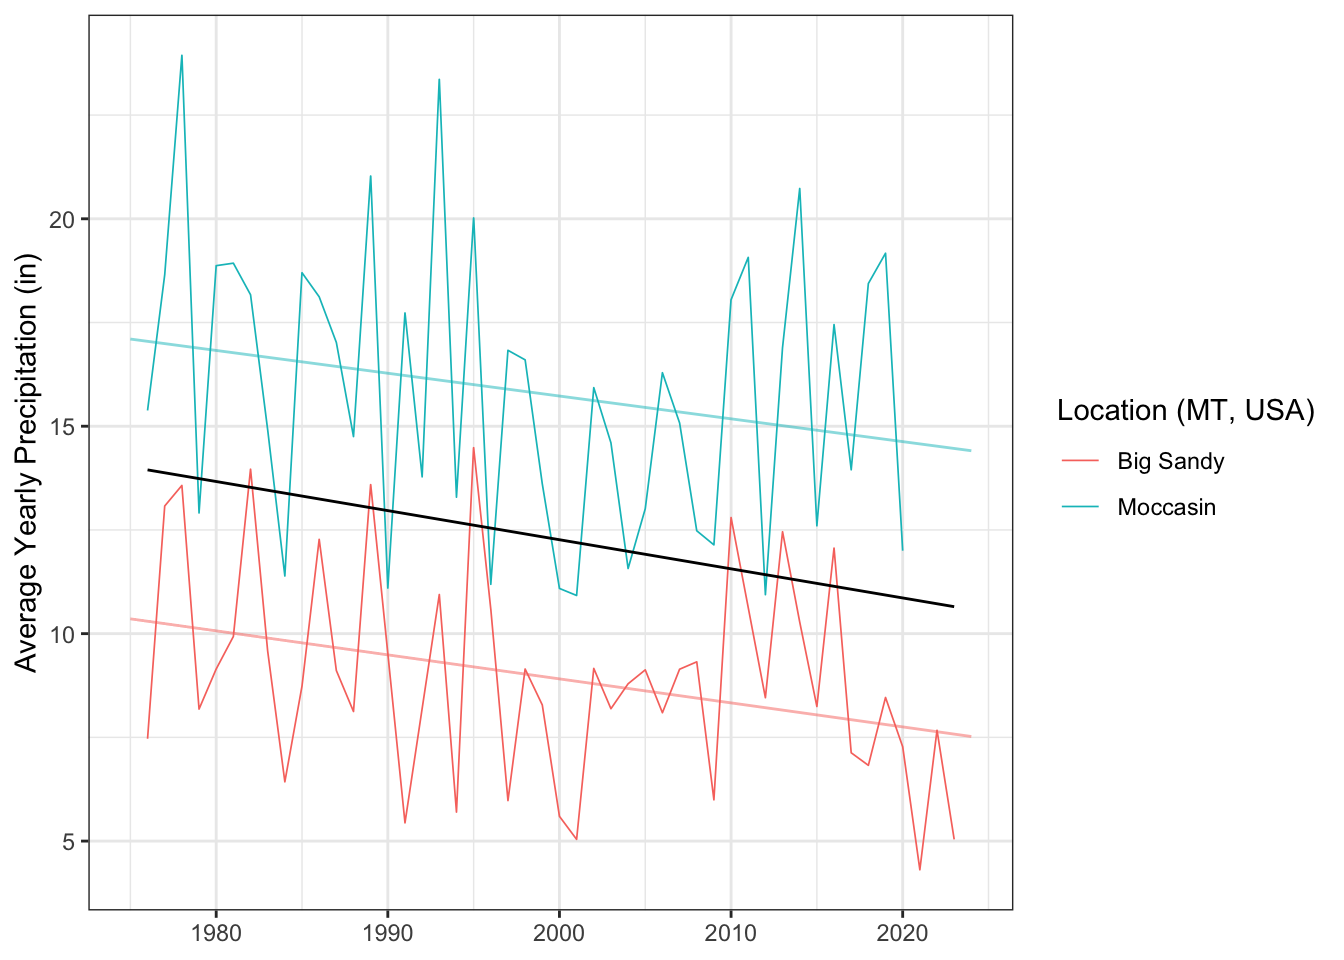
\includegraphics{JacksonStrand_Paper 1_files/figure-latex/FIG1_both_prcp_plot-1.pdf}
\caption{Figure 1: Average yearly precipitation (in) for Big Sandy and
Moccasin, Montana. Black trend line signifies averaged negative trend
between both locations. Data gathered from NOAA and MSU-ARS. A
significant linear relationship (r = 0.1, P = 0.033, estimate = -0.058)
was observed between year and average yearly precipitation.}
\end{figure}

\subsubsection{Figure 2}\label{figure2}

\begin{figure}
\centering
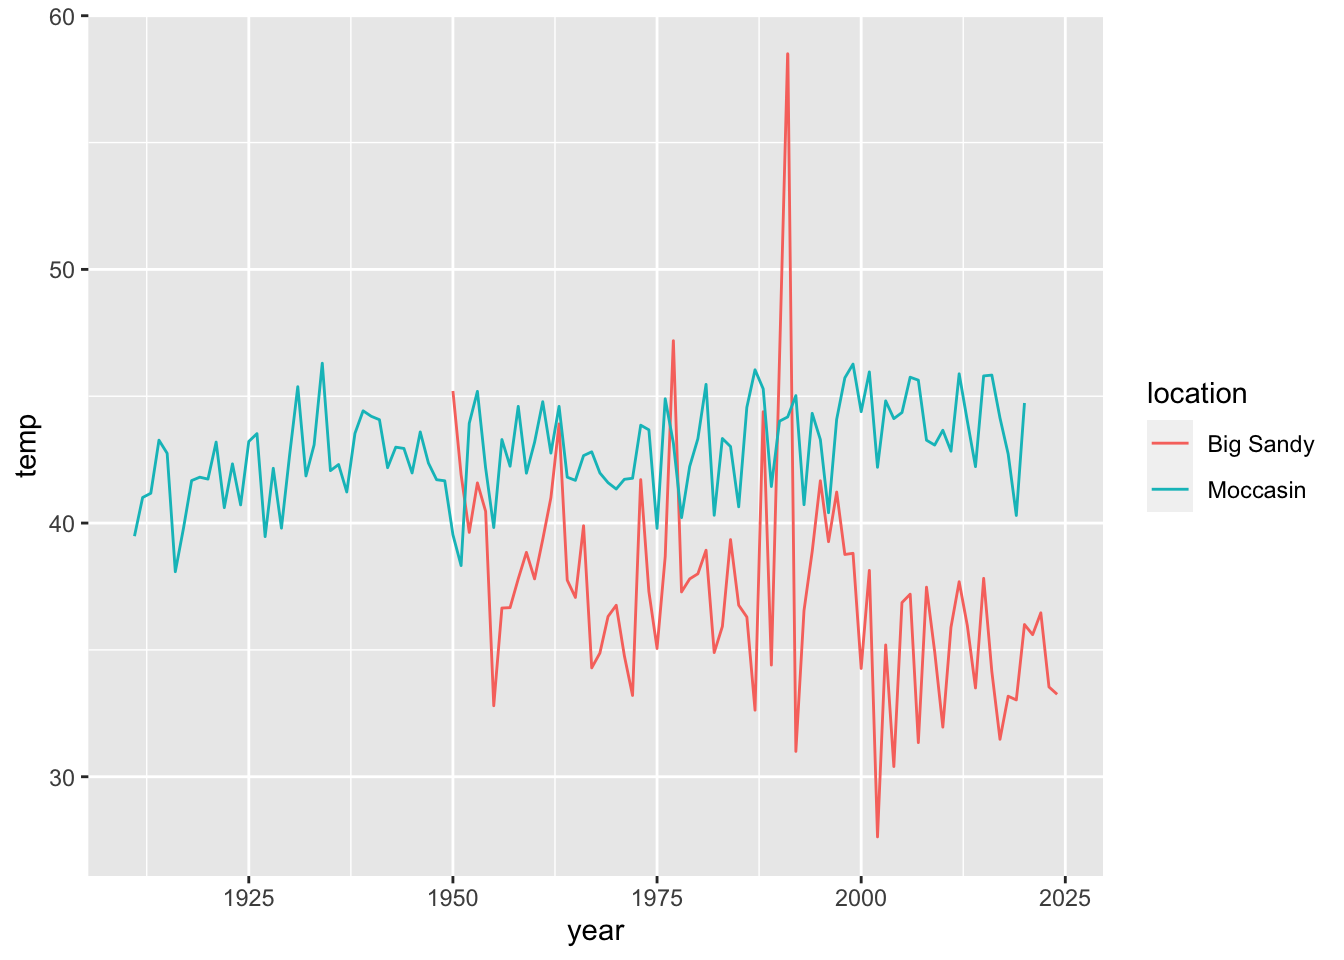
\includegraphics{JacksonStrand_Paper 1_files/figure-latex/both_temp_plot-1.pdf}
\caption{Figure 2: Average yearly temperature (°C) in Moccasin and Big
Sandy, MT. Positive trendline slop suggests increasing average
temperatures of the past 100 years. A significant linear relationship
(\emph{r =0.2447, P \textless{} 0.05, estimate = 0.028}) was observed
between year and average yearly temperature.}
\end{figure}

\subsubsection{Figure 3}\label{figure3}

\begin{figure}
\centering
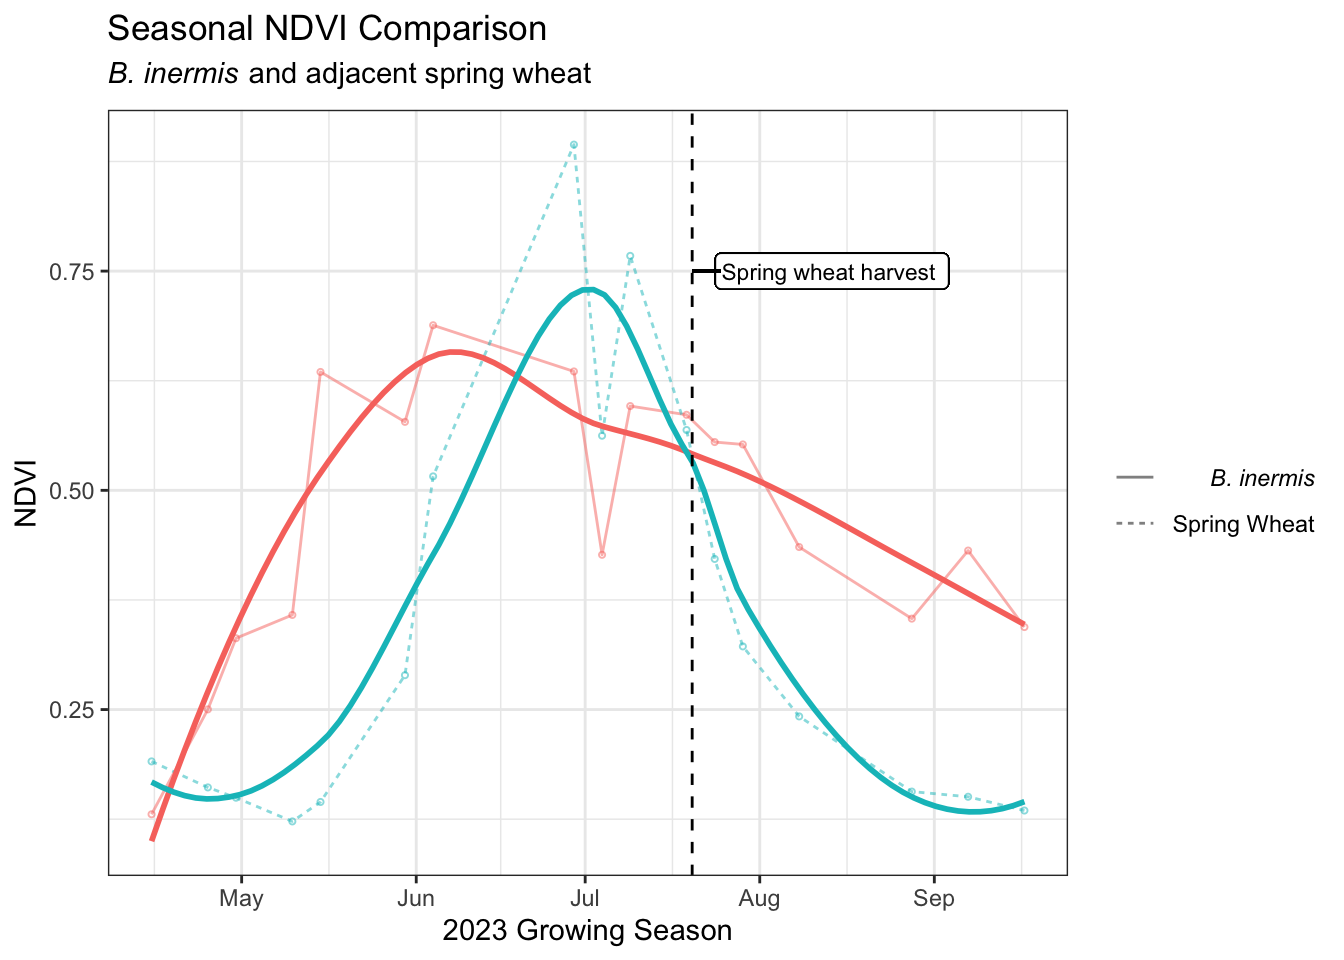
\includegraphics{JacksonStrand_Paper 1_files/figure-latex/bs_ndvi_plot-1.pdf}
\caption{Figure 3: Normalized difference vegetation index (NDVI) of
\emph{B. inermis} and adjacent spring wheat field from April 2023 to
October 2023. Post harvest linear model indicates a significant
difference (P values and stuff) when comparing the \emph{B. inermis}
post-harvest slope and the spring wheat post-harvest slope.}
\end{figure}

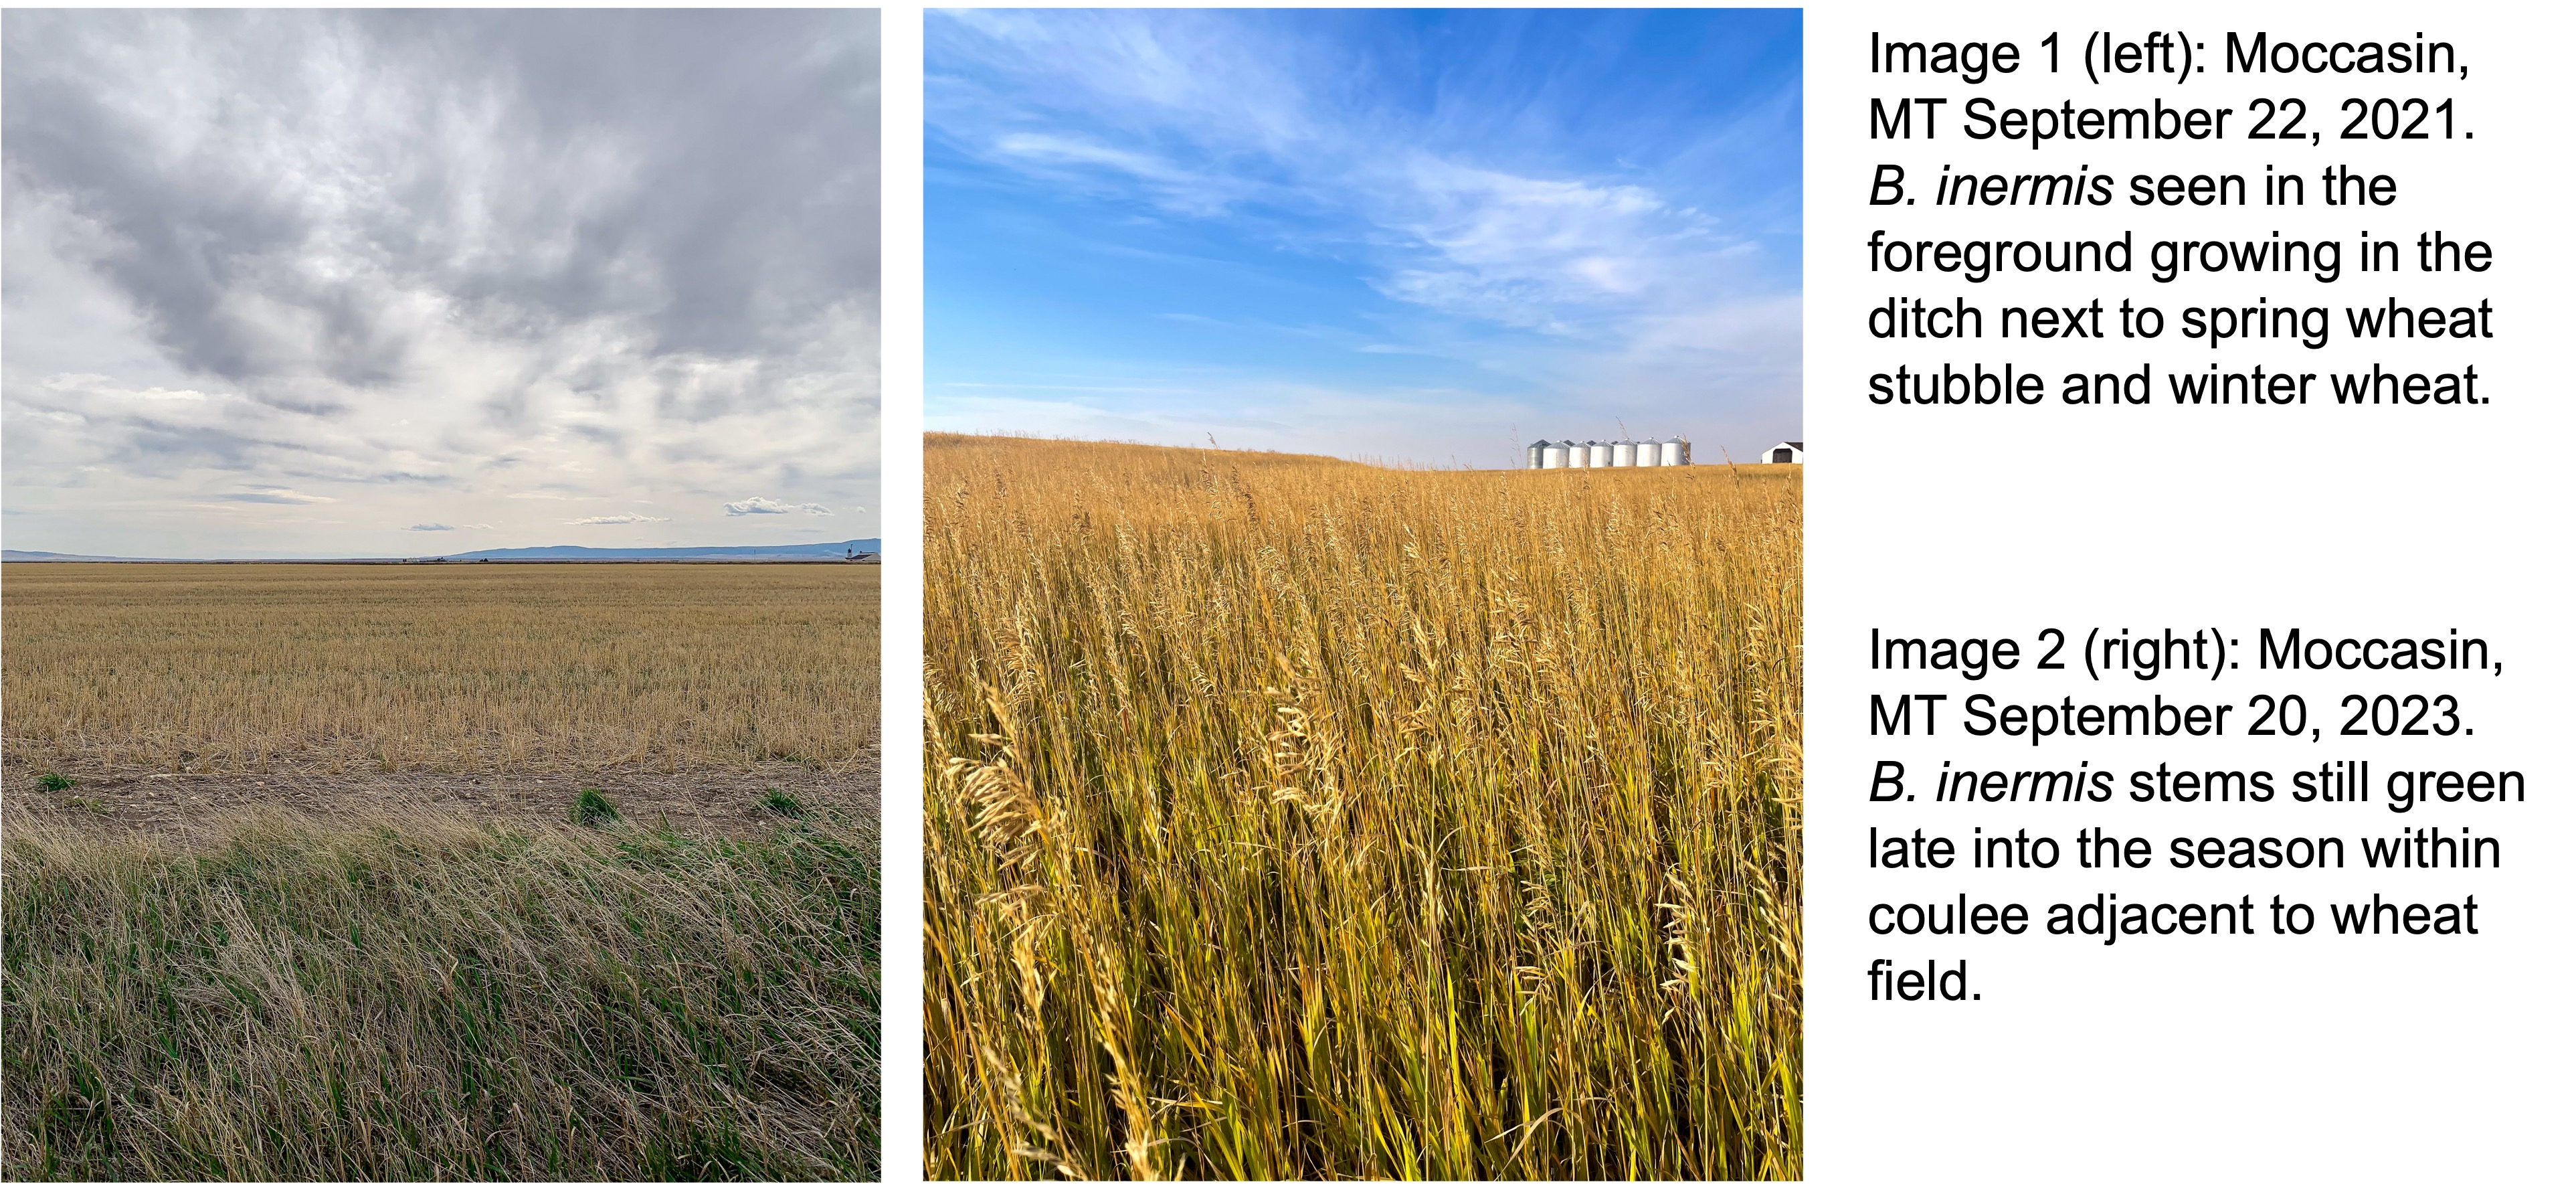
\includegraphics{Images/brome_images.jpg}

\subsubsection{Figure 4}\label{figure4}

\begin{figure}
\centering
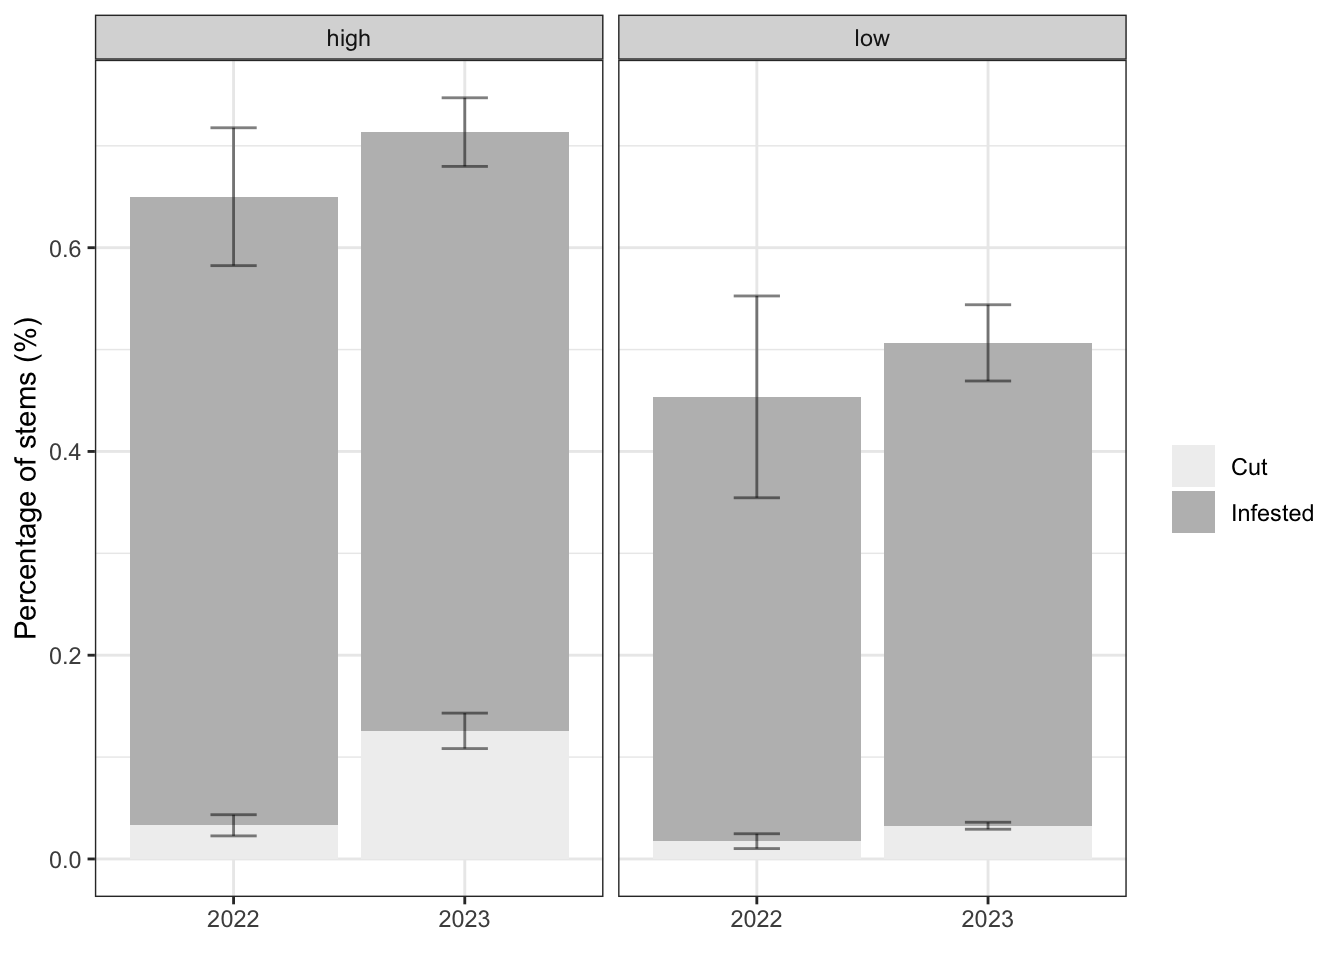
\includegraphics{JacksonStrand_Paper 1_files/figure-latex/inf_cut_plot-1.pdf}
\caption{Figure 4: Comparison of year and treatment group for controlled
infestation of \emph{B. inermis}. Three treatment groups - high, low,
and control (0) - were used. The controlled groups showed no sign of
\emph{C. cinctus} stem damage. We observed a significant difference in
cutting between high and low treatment groups (\emph{r = 0.592, P
\textless{} 0.05}).}
\end{figure}

\subsubsection{Figure 5}\label{figure5}

\begin{figure}
\centering
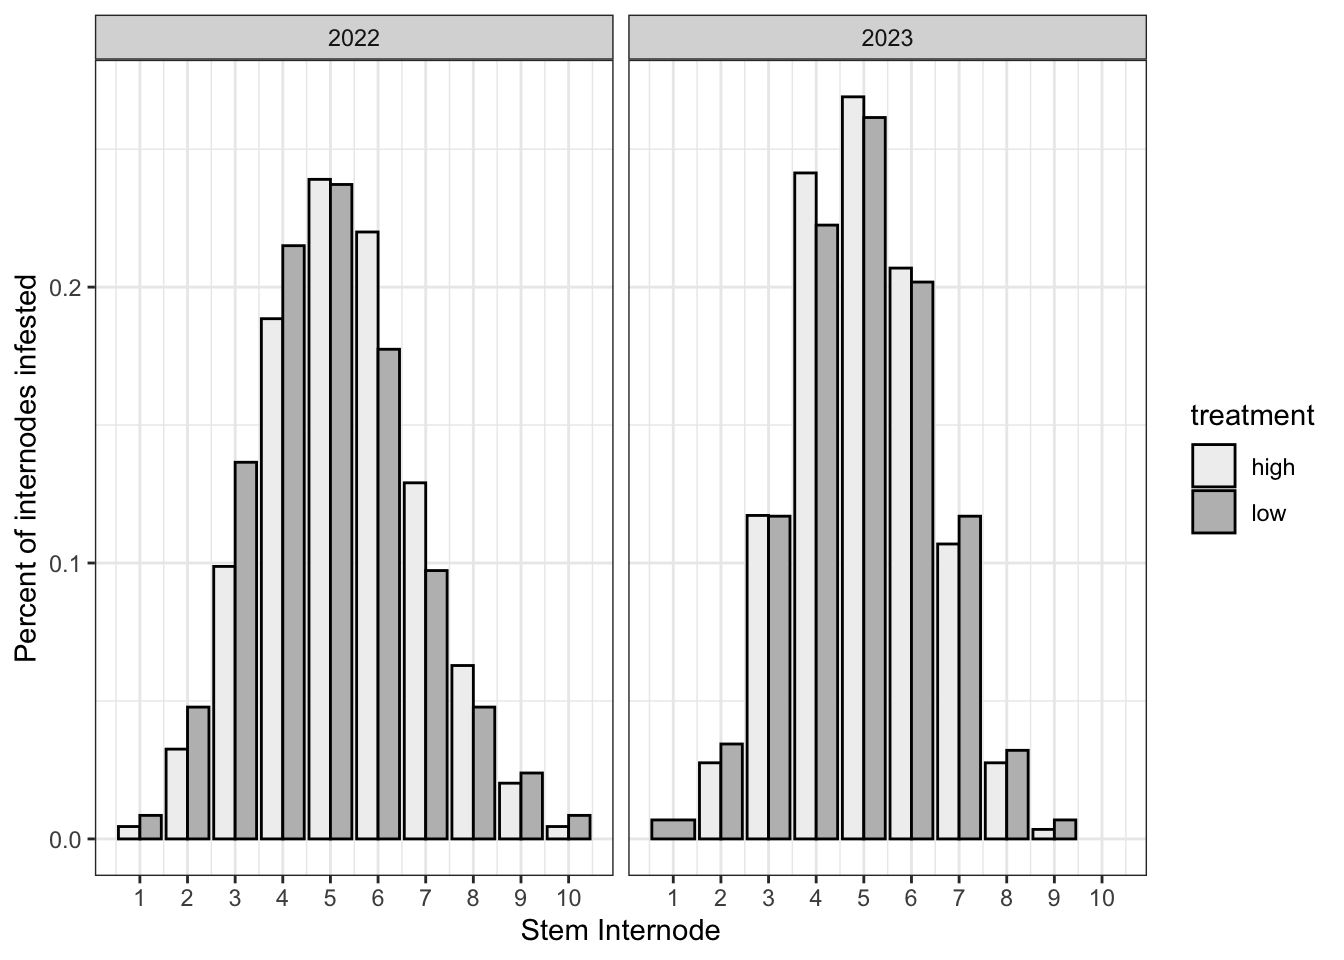
\includegraphics{JacksonStrand_Paper 1_files/figure-latex/figure5_pf_nodes_plot-1.pdf}
\caption{Figure 6: Ineternodes infested by \emph{B. cephi} within
controlled infestation plots in Bozeman, MT, USA. We found that 61.2\%
of stems exhibited infestation in at least 5 nodes}
\end{figure}

\subsubsection{Figure 6}\label{figure6}

\begin{figure}
\centering
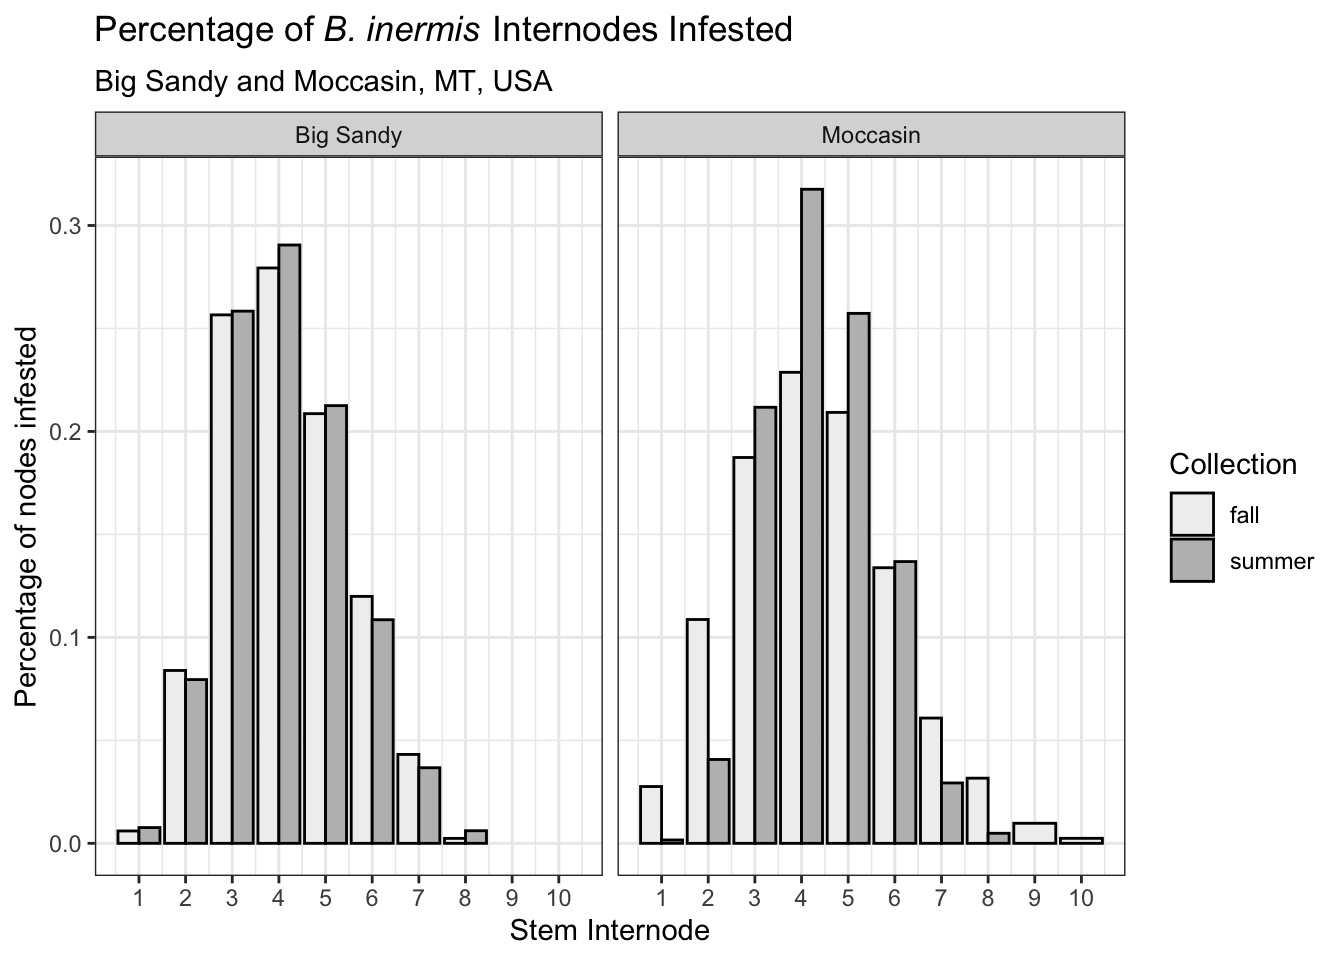
\includegraphics{JacksonStrand_Paper 1_files/figure-latex/figure6_brome_nodes-1.pdf}
\caption{Figure 6: Internodes infested by \emph{B. cephi} within
collected \emph{B. inermis} stems in Moccasin and Big Sandy, MT, USA.}
\end{figure}

\subsubsection{Figure 7}\label{figure7}

\begin{figure}
\centering
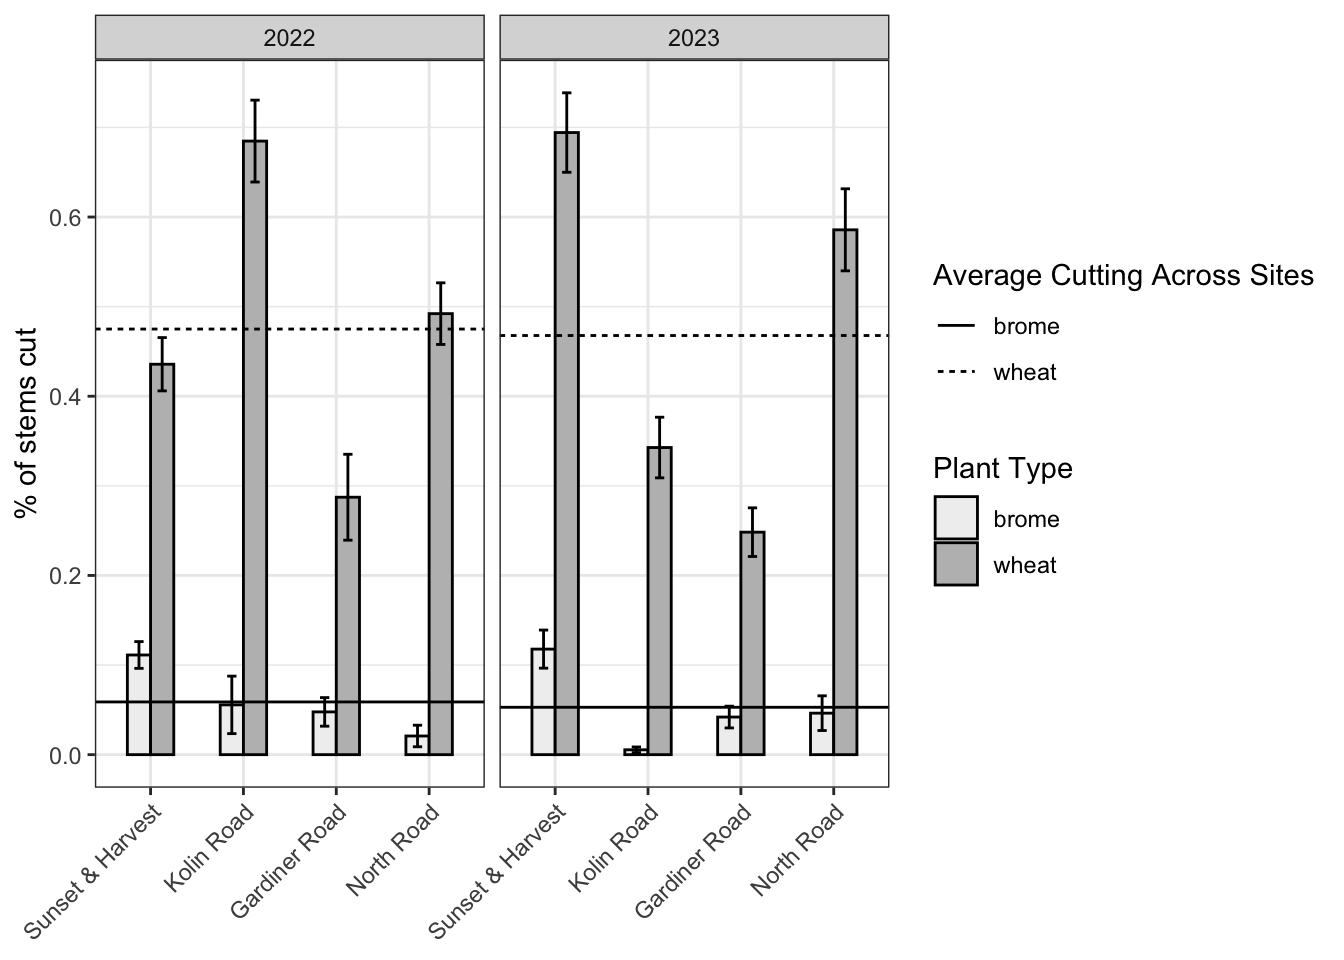
\includegraphics{JacksonStrand_Paper 1_files/figure-latex/figure7_field_cut_plot-1.pdf}
\caption{Figure 7: Stem cutting by \emph{C. cinctus}. We compared WSS
cutting in \emph{B. inermis} and adjacent wheat fields in Big Sandy and
Moccasin, MT, USA. The horizontal lines correspond to yearly mean
cutting for each plant type across all sampling sites.}
\end{figure}

\subsubsection{Figure 8}\label{figure8}

\begin{figure}
\centering
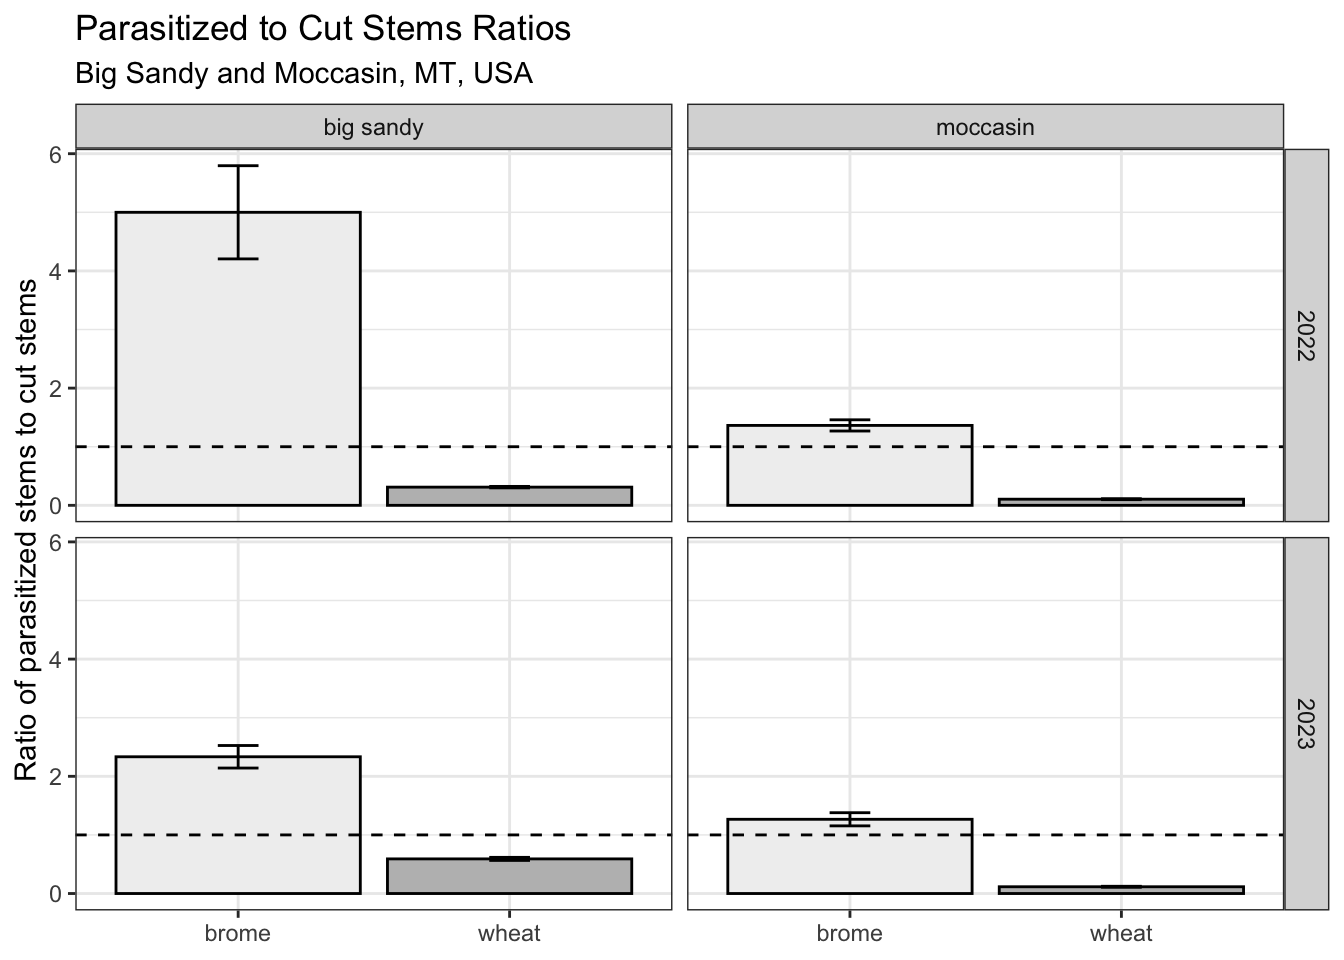
\includegraphics{JacksonStrand_Paper 1_files/figure-latex/figure8-1.pdf}
\caption{Ratios of parasitized to cut stems in \emph{B. inermis} and
adjacent cultivated wheat. Dotted line represents where a 1:1
cut:parasitized ratio lies.}
\end{figure}

\subsubsection{Figure 9}\label{figure9}

\begin{figure}

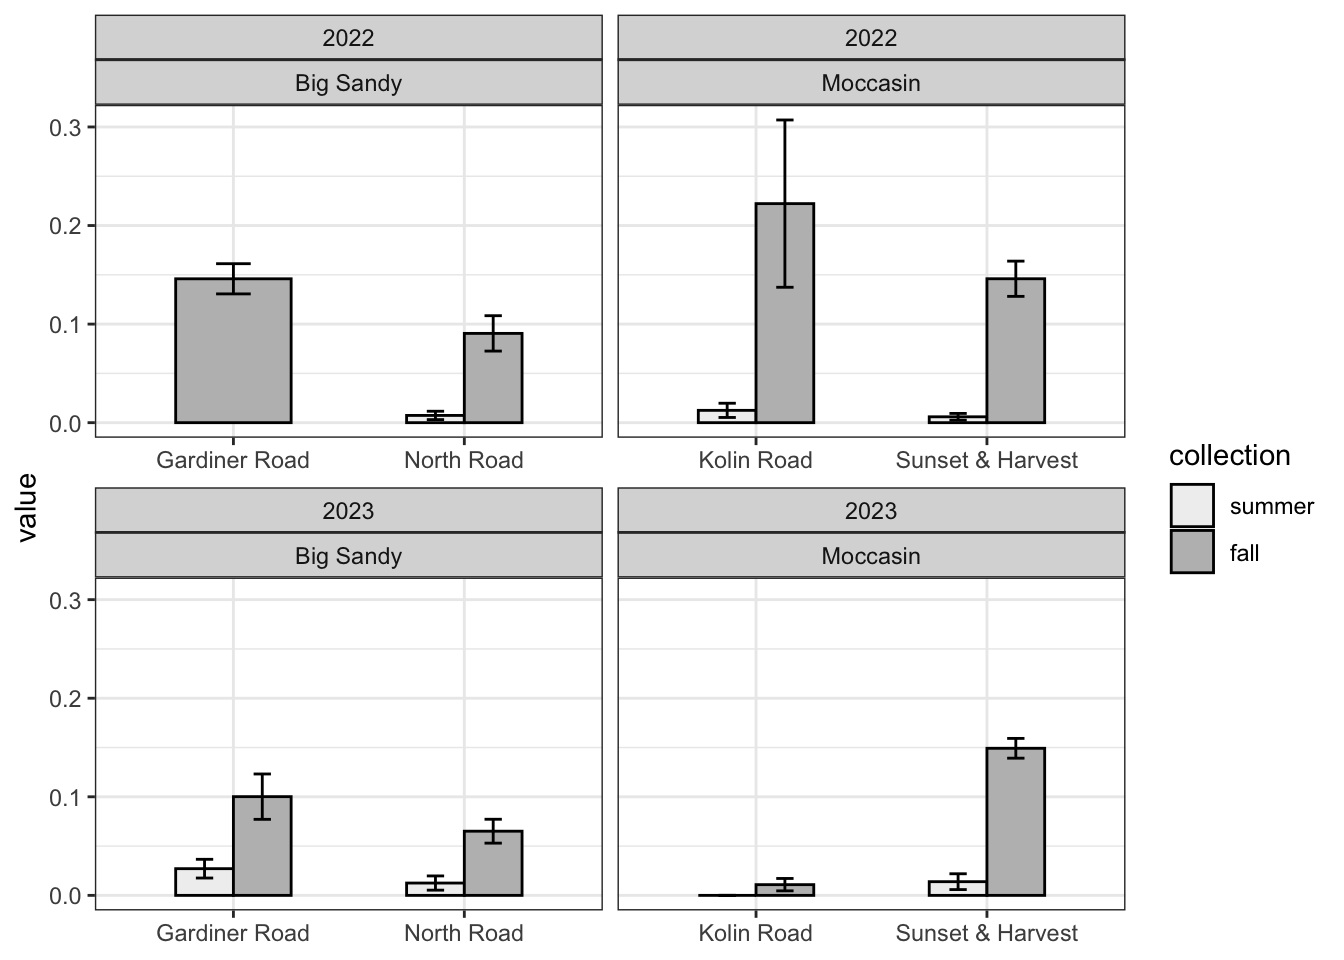
\includegraphics{JacksonStrand_Paper 1_files/figure-latex/figure9-1} \hfill{}

\caption{Comparison of parasitoid presence in *B. inermis* between July and September collections.}\label{fig:figure9}
\end{figure}

\subsubsection{Figure 10}\label{figurex}

\begin{figure}
\centering
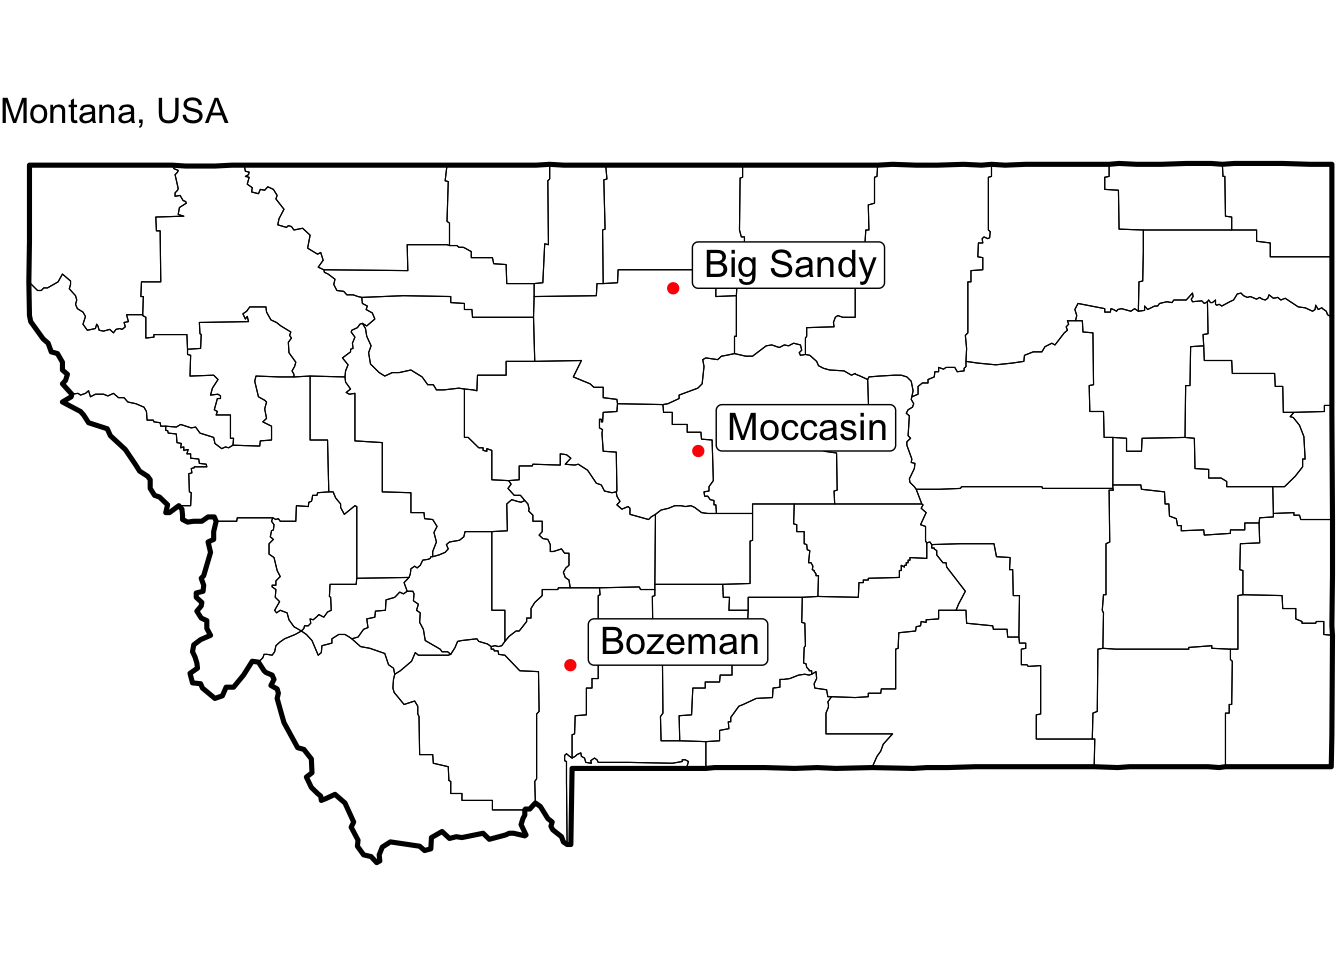
\includegraphics{JacksonStrand_Paper 1_files/figure-latex/figure10-1.pdf}
\caption{Location of Montana, USA field sites. Controlled \emph{B.
inermis} infestation site was in Bozeman, while field sites were located
in centrally location Moccasin, MT and northern Big Sandy, MT.}
\end{figure}

\subsection*{Citations}\label{citations}
\addcontentsline{toc}{subsection}{Citations}

\phantomsection\label{refs}
\begin{CSLReferences}{0}{1}
\bibitem[\citeproctext]{ref-Achhami2020}
Achhami BB, Reddy GVP, Sherman JD, et al. 2020. Antixenosis, antibiosis,
and potential yield compensatory response in barley cultivars exposed to
wheat stem sawfly (hymenoptera: Cephidae) under field conditions.
Journal of Insect Science. 20:1--14.
\url{https://doi.org/10.1093/JISESA/IEAA091}.

\bibitem[\citeproctext]{ref-Adhikari2019}
Adhikari S, Adhikari A, Weaver DK, et al. 2019. Impacts of agricultural
management systems on biodiversity and ecosystem services in highly
simplified dryland landscapes. Sustainability (Switzerland). 11.
\url{https://doi.org/10.3390/su11113223}.

\bibitem[\citeproctext]{ref-Ainslie1920}
Ainslie CN. 1920. The western grass-stem sawfly. United States
Department of Agriculture.

\bibitem[\citeproctext]{ref-lme4}
Bates MD, Bolker B, Walker S. 2015. Fitting linear mixed-effects models
using lme4. Journal of Statistical Software. 67:1--48.

\bibitem[\citeproctext]{ref-Bekkerman2018}
Bekkerman A, Weaver DK. 2018. Modeling joint dependence of managed
ecosystems pests: The case of the wheat stem sawfly. Journal of
Agricultural and Resource Economics. 43:172--194.

\bibitem[\citeproctext]{ref-Beres2011a}
Beres BL, Cárcamo HA, Weaver DK, et al. 2011. Integrating the building
blocks of agronomy and biocontrol into an IPM strategy for wheat stem
sawfly. Background and status. :54--65. Available from
\href{https://www.prairiesoilsandcrops.caVolume4·▪2011}{www.prairiesoilsandcrops.caVolume4·▪2011}.

\bibitem[\citeproctext]{ref-Beres2011}
Beres BL, Dosdall LM, Weaver DK, et al. 2011. Biology and integrated
management of wheat stem sawfly and the need for continuing research.
Canadian Entomologist. 143:105--125.
\url{https://doi.org/10.4039/n10-056}.

\bibitem[\citeproctext]{ref-Bhandari2020}
Bhandari R. 2020.
\href{https://www.ncbi.nlm.nih.gov/pubmed/25246403}{Assessment of host
selection behaviors and oviposition preferences of cephus cinctus norton
(hymenoptera: Cephidae) using wheat and smooth brome}.

\bibitem[\citeproctext]{ref-Buteler2015}
Buteler M, Peterson RKD, Hofland ML, et al. 2015. A multiple decrement
life table reveals that host plant resistance and parasitism are major
causes of mortality for the wheat stem sawfly. Environmental Entomology.
44:1571--1580. \url{https://doi.org/10.1093/ee/nvv128}.

\bibitem[\citeproctext]{ref-Buteler2008}
Buteler M, Weaver DK, Miller PR. 2008. Wheat stem sawfly-infested plants
benefit from parasitism of the herbivorous larvae. Agricultural and
Forest Entomology. 10:347--354.
\url{https://doi.org/10.1111/j.1461-9563.2008.00396.x}.

\bibitem[\citeproctext]{ref-Buteler2009}
Buteler M, Weaver DK, Peterson RKD. 2009. Oviposition behavior of the
wheat stem sawfly when encountering plants infested with cryptic
conspecifics. Journal of Environmental Entomology. 38:1707--1715.
Available from
\url{https://academic.oup.com/ee/article/38/6/1707/361666}.

\bibitem[\citeproctext]{ref-Cano2022}
Cano D, Martínez-Núñez C, Pérez AJ, et al. 2022. Small floral patches
are resistant reservoirs of wild floral visitor insects and the
pollination service in agricultural landscapes. Biological Conservation.
276. \url{https://doi.org/10.1016/j.biocon.2022.109789}.

\bibitem[\citeproctext]{ref-Carlson1985}
Carlson IT, Newell LC. 1985. Smooth bromegrass. In: Forages: the science
of grassland agriculture. Iowa State University. p. 198--206. Available
from \url{https://www.cabdirect.org/cabdirect/abstract/19850777665}.

\bibitem[\citeproctext]{ref-Cockrell2017}
Cockrell DM, Griffin-Nolan RJ, Rand TA, et al. 2017. Host plants of the
wheat stem sawfly (hymenoptera: cephidae). Environmental Entomology.
46:847--854. \url{https://doi.org/10.1093/ee/nvx104}.

\bibitem[\citeproctext]{ref-Cockrell2021}
Cockrell DM, Randolph T, Peirce E, et al. 2021. Survey of wheat stem
sawfly (hymenoptera: Cephidae) infesting wheat in eastern colorado.
Journal of Economic Entomology. 114:998--1004.
\url{https://doi.org/10.1093/JEE/TOAB015}.

\bibitem[\citeproctext]{ref-Criddle1922}
Criddle N. 1922. The western-stem sawfly and its control. Canadian
Department of Agriculture.

\bibitem[\citeproctext]{ref-Davis1955}
Davis EG, Benton C, Somsen HW. 1955. Natural enemies of the wheat stem
sawfly in north dakota and montana. North Dakota Agricultural
Experimental Bimonthly Bulletin. 18:63--65.

\bibitem[\citeproctext]{ref-Davis2013}
Davis RA. 2013. Mechanisms for reproductive isolation in two congeneric
parasitoids of the wheat stem sawfly.

\bibitem[\citeproctext]{ref-Dillemuth2008}
Dillemuth FP, Rietschier EA, Cronin JT. 2008. Patch dynamics of a native
grass in relation to the spread of invasive smooth brome
(bromus~inermis). Biological Invasions 2008 11:6. 11:1381--1391.
\url{https://doi.org/10.1007/S10530-008-9346-7}.

\bibitem[\citeproctext]{ref-Evans1999}
Evans EW. 1999. Intra versus interspecific interactions of ladybeetles
(coleoptera: Coccinellidae) attacking aphids.

\bibitem[\citeproctext]{ref-Farstad1945}
Farstad CW, Jacobson L. 1945. Manual for sawfly control workers in
alberta.

\bibitem[\citeproctext]{ref-Gahan1918}
Gahan AB. 1918. Description of a new hymenopterous parasite
(braconidae). In: Proceedings of the Entomological Society of
Washington. Vol. 20. p. 18--19.

\bibitem[\citeproctext]{ref-Hager2024}
Hager MS, Hofland ML, Varella AC, et al. 2024. Untargeted metabolomics
profiling of oat (avena sativa l.) and wheat (triticum aestivum l.)
infested with wheat stem sawfly (cephus cinctus norton) reveals
differences associated with plant defense and insect nutrition.
Frontiers in Plant Science. 15.
\url{https://doi.org/10.3389/fpls.2024.1327390}.

\bibitem[\citeproctext]{ref-Holmes1982}
Holmes ND. 1982. Population dynamics of the wheat stem sawfly. The
Canadian Entomologist. 114:775--788.
\url{https://doi.org/10.4039/Ent114775-9}.

\bibitem[\citeproctext]{ref-Holmes1956}
Holmes ND, Farstad CW. 1956. Effects of field exposure on immature
stages of the wheat stem sawfly, cephus cinctus nort. (Hymenoptera:
cephidae). Canadian Journal of Agricultural Science. 36:196--202.
Available from
\url{https://cdnsciencepub.com/doi/abs/10.4141/agsci-1956-0023}.

\bibitem[\citeproctext]{ref-Holmes1963}
Holmes ND, Nelson WA, Peterson LK, et al. 1963. Causes of variation in
effectiveness of bracon cephi (gahan) (hymenoptera: Braconidae) as a
parasite of the wheat stem sawfly. The Canadian Entomologist.
95:113--126.

\bibitem[\citeproctext]{ref-Holmes1960}
Holmes ND, Peterson LK. 1960. THE INFLUENCE OF THE HOST ON OVIPOSITION
BY THE WHEAT STEM SAWFLY, CEPHUS CINCTUS NORT. (HYMENOPTERA: CEPHIDAE).
Canadian Journal of Plant Science. 40:29--46.
\url{https://doi.org/10.4141/cjps60-004}.

\bibitem[\citeproctext]{ref-Kennedy2000}
Kennedy GG, Storer NP. 2000. Life systems of polyphagous arthropod pests
in temporally unstable cropping systems. Annual Review of Entomology.
45:467--493.

\bibitem[\citeproctext]{ref-Lesieur2016}
Lesieur V, Martin JF, Weaver DK, et al. 2016. Phylogeography of the
wheat stem sawfly, cephus cinctus norton (hymenoptera: Cephidae):
Implications for pest management. PLoS ONE. 11:168370.
\url{https://doi.org/10.1371/journal.pone.0168370}.

\bibitem[\citeproctext]{ref-McCullough2020}
McCullough CT, Hein GL, Bradshaw JD. 2020. Phenology and dispersal of
the wheat stem sawfly (hymenoptera: Cephidae) into winter wheat fields
in nebraska. Journal of Economic Entomology. 113:1831--1838.
\url{https://doi.org/10.1093/jee/toaa093}.

\bibitem[\citeproctext]{ref-DeMorais2023}
Morais RMD, Freitas De Morais A de, Handte VG, et al. 2023. Enhancing
arthropod communities through plant diversified edge of kale
cultivation. Pesquisa Agropecuária Gaúcha. 29:77--91.
\url{https://doi.org/10.36812/pag.202329177-91}.

\bibitem[\citeproctext]{ref-Morrill1996}
Morrill WL, Kushnak GD. 1996. Wheat stem sawfly (hymenoptera: Cephidae)
adaptation to winter wheat. Environmental Entomology. 25:1128--1132.
\url{https://doi.org/10.1093/EE/25.5.1128}.

\bibitem[\citeproctext]{ref-Morrill1998}
Morrill WL, Kushnak GD, Gabor JW. 1998. Parasitism of the wheat stem
sawfly (hymenoptera: Cephidae) in montana. Biological Control.
12:159--163. \url{https://doi.org/10.1006/bcon.1998.0629}.

\bibitem[\citeproctext]{ref-Morrill2001}
Morrill WL, Weaver DK, Johnson GD. 2001. Trap strip and field border
modification for management of the wheat stem sawfly (hymenoptera:
cephidae). Journal of Entomological Science. 36:34--45.
\url{https://doi.org/10.18474/0749-8004-36.1.34}.

\bibitem[\citeproctext]{ref-Nansen2005a}
Nansen C, Macedo TB, Weaver DK, et al. 2005. Spatiotemporal
distributions of wheat stem sawfly eggs and larvae in dryland wheat
fields. Canadian Entomologist. 137:428--440.
\url{https://doi.org/10.4039/n04-094}.

\bibitem[\citeproctext]{ref-Nelson1953}
Nelson WA, Farstad CW. 1953. Biology of bracon cephi (gahan)
(hymenoptera: Braconidae), an important native parasite of the wheat
stem sawfly, cephus cinctus nort. (Hymenoptera: Cephidae), in western
canada. The Canadian Entomologist. 85:103--107.
\url{https://doi.org/10.4039/Ent85103-3}.

\bibitem[\citeproctext]{ref-Olfert2019}
Olfert O, Weiss RM, Catton H, et al. 2019. Bioclimatic assessment of
abiotic factors affecting relative abundance and distribution of wheat
stem sawfly (hymenoptera: Cephidae) in western canada. Canadian
Entomologist. 151:16--33. \url{https://doi.org/10.4039/tce.2018.46}.

\bibitem[\citeproctext]{ref-Otfinowski2006}
Otfinowski R, Kenkel NC, Catling PM. 2006. The biology of canadian
weeds. 134. Bromus inermis leyss. Canadian Journal of Plant Science.
87:183--198.

\bibitem[\citeproctext]{ref-Pederson2009}
Pederson GT, Graumlich LJ, Fagre DB, et al. 2009. A century of climate
and ecosystem change in western montana: What do temperature trends
portend? Climatic Change. 98:133--154.
\url{https://doi.org/10.1007/s10584-009-9642-y}.

\bibitem[\citeproctext]{ref-Peirce2021}
Peirce ES, Rand TA, Cockrell DM, et al. 2021. Effects of landscape
composition on wheat stem sawfly (hymenoptera: Cephidae) and its
associated braconid parasitoids. Journal of Economic Entomology.
114:72--81. \url{https://doi.org/10.1093/jee/toaa287}.

\bibitem[\citeproctext]{ref-Mendoza2006}
Perez-Mendoza J, Weaver DK. 2006. Temperature and relative humidity
effects on postdiapause larval development and adult emergence in three
populations of wheat stem sawfly (hymenoptera: cephidae). Environmental
Entomology. 35:1222--1231. \url{https://doi.org/10.1093/ee/35.5.1222}.

\bibitem[\citeproctext]{ref-Peterson2011}
Peterson RKD, Buteler M, Weaver DK, et al. 2011. Parasitism and the
demography of wheat stem sawfly larvae, cephus cinctus. BioControl.
56:831--839. \url{https://doi.org/10.1007/s10526-011-9357-7}.

\bibitem[\citeproctext]{ref-Peterson1999}
Peterson RO. 1999. Wolf-moose interaction on isle royale: The end of
natural regulation. Ecological Applications. 9:10--16.
\url{https://doi.org/10.1890/1051-0761(1999)009\%5B0010:WMIOIR\%5D2.0.CO;2}.

\bibitem[\citeproctext]{ref-Pettorelli2005}
Pettorelli N, Vik JO, Mysterud A, et al. 2005. Using the
satellite-derived NDVI to assess ecological responses to environmental
change. Trends in Ecology and Evolution. 20:503--510.
\url{https://doi.org/10.1016/j.tree.2005.05.011}.

\bibitem[\citeproctext]{ref-Rand2024}
Rand TA, Kula RR, Gaskin JF. 2024. Evaluating the use of common grasses
by the wheat stem sawfly (hymenoptera: Cephidae) and its native
parasitoids in rangeland and conservation reserve program grasslands.
Liu T-X, editor. Journal of Economic Entomology.
\url{https://doi.org/10.1093/jee/toae046}.

\bibitem[\citeproctext]{ref-Rand2020}
Rand TA, Richmond CE, Dougherty ET. 2020. Modeling the combined impacts
of host plant resistance and biological control on the population
dynamics of a major pest of wheat. Pest Management Science.
76:2818--2828. \url{https://doi.org/10.1002/ps.5830}.

\bibitem[\citeproctext]{ref-Runyon2001b}
Runyon JB. 2001. Wheat stem sawfly parasitism in varying field sizes and
tillage systems in dryland wheat in montana. Canadian Entomologist. 133.

\bibitem[\citeproctext]{ref-Runyon2001a}
Runyon JB, Hurley RL, Morrill WL, et al. 2001. Distinguishing adults of
bracon cephi and bracon lissogaster (hymenoptera: Braconidae),
parasitoids of the wheat stem sawfly (hymenoptera: cephidae). Canadian
Entomologist. 133:215--217. \url{https://doi.org/10.4039/Ent133215-2}.

\bibitem[\citeproctext]{ref-Runyon2002}
Runyon JB, Morrill WL, Weaver DK, et al. 2002. Parasitism of the wheat
stem sawfly (hymenoptera: Cephidae) by bracon cephi and b. Lissogaster
(hymenoptera: Braconidae) in wheat fields bordering tilled and untilled
fallow in montana. Journal of economic entomology. 95:1130--1134.
\url{https://doi.org/10.1603/0022-0493-95.6.1130}.

\bibitem[\citeproctext]{ref-Bolwahn2011}
Salesman JB, Thomsen M. 2011. Smooth brome (bromus inermis) in tallgrass
prairies: A review of control methods and future research directions.
Ecological Restoration. 29:374--381.
\url{https://doi.org/10.3368/er.29.4.374}.

\bibitem[\citeproctext]{ref-Seamans1928}
Seamans HL. 1928. The value of trap crops in the control of the wheat
stem sawfly in alberta. The Value of Trap Crops in the Control of the
Wheat Stem Sawfly in Alberta.

\bibitem[\citeproctext]{ref-Shanower2004}
Shanower TG, Hoelmer KA. 2004. Biological control of wheat stem
sawflies: Past and future. Journal of Agricultural Entomology.
21:197--221.

\bibitem[\citeproctext]{ref-Somsen1956}
Somsen HW, Luginbill P. 1956. Bracon lissogaster mues: A parasite of the
wheat stem sawfly. USDA Technical Bullitin. 1153. Available from
\url{https://www.google.com/books/edition/Bracon_Lissogaster_Mues/37UXAAAAYAAJ?hl=en&gbpv=1&dq=Bracon+Lissogaster+Mues:+A+Parasite+of+the+Wheat+Stem+Sawfly.&pg=PA29&printsec=frontcover}.

\bibitem[\citeproctext]{ref-Tscharntke2016}
Tscharntke T, Karp DS, Chaplin-Kramer R, et al. 2016. When natural
habitat fails to enhance biological pest control -- five hypotheses.
Biological Conservation. 204:449--458.
\url{https://doi.org/10.1016/j.biocon.2016.10.001}.

\bibitem[\citeproctext]{ref-Villacorta1971}
Villacorta A, Bell R, Callenbach J. 1971. Influence of high temperature
and light on postdiapause development of the wheat stem sawfly. Journal
of Economic Entomology. 64:749--751.

\bibitem[\citeproctext]{ref-Wallace1966}
Wallace LE, McNeal FH. 1966. Stem sawflies of economic importance in
grain crops in the united states. U.S. Department of Agriculture
Technical Bulletin No. 1350. Available from
\href{https://books.google.com/books?hl=en&lr=&id=dcMXAAAAYAAJ&oi=fnd&pg=PA1&dq=Stem+sawflies+of+economic+importance+in+grain+crops+in+the+United+States&ots=e0FbKZOb6x&sig=_fPd1FCRZ_HK-Ncv2POX-EFMvOo\#v=onepage&q=Stem\%20sawflies\%20of\%20economic\%20importance\%20in\%20grain\%20cro}{https://books.google.com/books?hl=en\&lr=\&id=dcMXAAAAYAAJ\&oi=fnd\&pg=PA1\&dq=Stem+sawflies+of+economic+importance+in+grain+crops+in+the+United+States\&ots=e0FbKZOb6x\&sig=\_fPd1FCRZ\_HK-Ncv2POX-EFMvOo\#v=onepage\&q=Stem
sawflies of economic importance in grain cro}.

\bibitem[\citeproctext]{ref-Weaver2023}
Weaver D. 2023. Wheat stem sawfly (cephus cinctus norton). p. 93--134.
\url{https://doi.org/10.19103/as.2022.0114.13}.

\bibitem[\citeproctext]{ref-ggplot}
Wickham H. 2016. ggplot2: Elegant graphics for data analysis. Available
from \url{https://ggplot2.tidyverse.org}.

\bibitem[\citeproctext]{ref-Willson2000}
Willson GD, Stubbendieck J. 2000. A provisional model for smooth brome
management in degraded tallgrass prairie. Ecological Restoration.
18:34--38. \url{https://doi.org/10.3368/er.18.1.34}.

\bibitem[\citeproctext]{ref-Wilson1923}
Wilson ML. 1923. Dry farming in the north central montana triangle.
Bowden RB, editor.

\bibitem[\citeproctext]{ref-Zhu2021}
Zhu P, Burney J. 2021. Temperature-driven harvest decisions amplify US
winter wheat loss under climate warming. Global Change Biology.
27:550--562. \url{https://doi.org/10.1111/gcb.15427}.

\end{CSLReferences}

\end{document}
